\documentclass[%
  corpo=12pt,
  tipotesi=magistrale,
  evenboxes,
  %libro,
  twoside
]{toptesi}

%%% Font %%%
\usepackage[utf8]{inputenc}
\usepackage[T1]{fontenc}
%\usepackage{newtxtext}% o altro font
\usepackage{amsmath}
\usepackage{amssymb}
\usepackage{inconsolata}

%%% Colors %%%
\usepackage[dvipsnames,svgnames,x11names,hyperref,table]{xcolor}

%%% Shorthand commands %%%
\usepackage{xspace}
\newcommand{\ooo}{out-of-order\xspace}
\newcommand{\riscv}{RISC-V\xspace}
\newcommand{\lens}{LEN5\xspace}

%%% Set paragraph spacing %%%
\setlength{\parskip}{0pt}

%%% Hyperref %%%
\usepackage{hyperref}
\hypersetup{%
    pdfpagemode={UseOutlines},
    bookmarksopen,
    pdfstartview={FitH},
    colorlinks,
    linkcolor={NavyBlue},
    citecolor={NavyBlue},
    urlcolor={blue}
  }

%%% Nice tables %%%
\usepackage{booktabs}

%%% Acronyms %%%
\usepackage[printonlyused,nohyperlinks]{acronym}

%%% Utils (can be removed at the end) %%%
\usepackage{lipsum}
\usepackage{todonotes}

\begin{document}
\english 

%%% Front matter %%%
\CorsoDiLaureaIn{Master's Degree in}
\TesiDiLaurea{Master Thesis}
\CandidateName{Candidate}
\AdvisorName{Supervisor}

\begin{frontespizio}
    %\ateneo{Politecnico di Torino}
    \logosede[30mm]{img/polito_logo.png}
    \corsodilaurea{Electronic Engineering}
    \titolo{Design of the frontend for LEN5, a RISC-V Out-of-Order processor}
    %\sottotitolo{Sottotitolo}
    \relatore{Prof. Maurizio \textsc{Martina}}
    \sedutadilaurea{Academic year 2018-2019}
    \candidato{Marco \textsc{Andorno}}    
\end{frontespizio}

%%% Abstract %%%
\begin{abstract}
\riscv is a free and open source Instruction Set Architecture, which has sparked interest all over the community of computer architects, as it paves the way for a previously unseen era of extensible software and hardware design freedom. One of its main strength points is the vast modularity implemented in terms of different ISA extensions, which aim to cover a very broad range of applications. This allows designers to tailor the architecture according to their specific needs, without constraining them to support unnecessary instructions.

Being \riscv a relatively new ISA, a limited number of cores is available at the moment, and in particular very few of them are open sourced. So the main motivation for this work is the contribution to this open source hardware community, by means of the design of an Out-of-Order \riscv core as general purpose as possible.

The core is a 64-bit processor, supporting the G extension, which is a short- hand for the base integer (I), multiply and divide (M), floating point (F) and atomic (A) extensions. One goal of this project, which will be carried out alongside two colleagues, is to eventually include support also for the operating system, by implementing the yet unstandardized Privileged ISA, for the experimental vector extension (V) and possibly for a matrix extension to be defined from scratch. These last design choices are motivated by the lack of open source cores supporting them, and the great advantage that such vectorized computation can provide in a world where the popularity and the performance needs of artificial intelligence and machine learning are ever-growing.

Moreover, the choice of designing an \ooo core arises mainly as all modern processors are of such kind, as it has been the best compromise to efficiently exploit instruction level parallelism for decades. The goal is to implement both instruction issue and execution to be performed Out-of-Order, because this allows the highest performance gain. This design choice, of course, comes with a series of implications that will need accurate analysis and bench- marking, possibly by keeping everything as parametric and modular as possible: branch prediction, instruction queue management, memory hierarchy and cache organization are just some examples.

The final outcome of this work will be an in-depth exploration of the design space offered by such complex architectures, to actually experience firsthand the main issues and tradeoffs designers must face and to be prepared to offer a significant contribution to the state of the art of processor design. Moreover, the common hope is for this project to serve as the basis for future in-house development of a complete \riscv-based platform here at Politecnico di Torino. As mentioned above, the entire work will be open source and available on a GitHub repository.
\end{abstract}

%%% Acknowledgements %%%
\ringraziamenti
Thanks everybody!

%%% Indices %%%
\figurespagetrue
\tablespagetrue
\indici
\chapter*{List of Acronyms}
\addcontentsline{toc}{chapter}{List of Acronyms}
\begin{acronym}[AAAA]
  \acro{ALU}{Arithmetic-Logic Unit}
  \acro{ASIC}{Application Specific Integrated Circuit}
  \acro{BHT}{Branch History Table}
  \acro{CDB}{Common Data Bus}
  \acro{CPI}{Clocks Per Instruction}
  \acro{CPU}{Central Processing Unit}
  \acro{FPGA}{Field Programmable Gate Array}
  \acro{FPU}{Floating Point Unit}
  \acro{IC}{Instruction Count}
  \acro{ILP}{Instruction-Level Parallelism}
  \acro{IPC}{Instructions Per Clock}
  \acro{ISA}{Instruction Set Architecture}
  \acro{PC}{Program Counter}
  \acro{PHT}{Pattern History Table}
  \acro{RAW}{Read-After-Write}
  \acro{ROB}{Reorder Buffer}
  \acro{TAGE}{Tagged Geometric}
  \acro{VLIW}{Very Long Instruction Word}
  \acro{WAR}{Write-After-Read}
  \acro{WAW}{Write-After-Write}
  \acro{WOE}{Window Of Execution}
\end{acronym}

%%% Chapters %%%
\chapter{Introduction}
\lipsum[1-3]
\chapter{State-of-the-art processor architectures}
The performance of a processor is defined by the the time it takes to execute a program. This time span, called \emph{\acsu{CPU} time}, can be expressed as:

\begin{equation*}
  \text{CPU time} = \frac{\text{Seconds}}{\text{Program}} = \frac{\text{Clock cycles}}{\text{Program}} \cdot T_{ck}
\end{equation*}
where $T_{ck}$ is the clock period.

The first term can be decomposed further by computing the total number of instructions inside a program, called \acfi{IC}, which is known given the assembly code of the program. From this figure and the total number of clock cycles, the average number of \acfi{CPI}\footnote{Sometimes, also the inverse figure can be used, that is \acfi{IPC}.} can be derived. By factoring in these quantities, the final expression of \ac{CPU} time is as follows \cite[p.~53]{hennessy17}:

\begin{equation}\label{eq:perf}
  \text{CPU time} = \text{IC} \cdot \text{CPI} \cdot T_{ck} 
\end{equation}

Equation \eqref{eq:perf} shows that the processor performance is directly and equally dependent on three factors:
\begin{itemize}
  \item Clock period, which depends mainly on the implementation technology and the microarchitectural choices (e.g. pipeline depth).
  \item \acsu{IC}, which is determined for the most part by the \ac{ISA} (see section \ref{sec:isas}) and compiler technology.
  \item \acsu{CPI}, which is dependant on both the \ac{ISA} and the architecture.
\end{itemize}
The goal is then to minimize each of these terms, but it is evident that none of these parameters can be modified without affecting the others, as many design choices influence many of them.

\section{Instruction-level parallelism}\label{sec:ilp}
Earliest processors executed instructions one at a time, fetching a new one only after the previous has finished, leading to a number of clock cycles per instruction greater than one, and in particular equal to the number of stages an instruction must get through. These processors, where $\text{CPI} > 1$, are called \emph{subscalar}. To illustrate the situation, in the example of the classic 5-stage RISC pipeline (fetch, decode, execute, memory access, write back), a subscalar processor would execute three consecutive instructions as shown in figure \ref{fig:subscalar}, taking a total of 15 clock cycles.

\begin{figure}[hbtp]
  \centering
  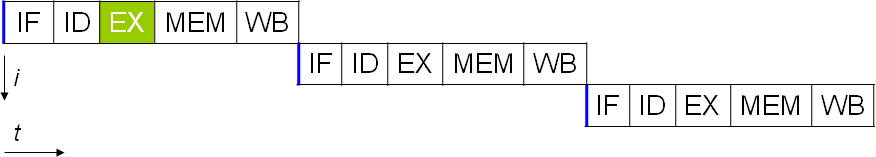
\includegraphics[width=0.8\textwidth]{img/subscalar.png}
  \caption{Subscalar processor}
  \label{fig:subscalar}
\end{figure}

Starting from the mid 80s, processor architects introduced \emph{pipelining} to improve performance by overlapping the execution of different instructions. This overlap means that at any given point in time there can be multiple instructions running in different stages of the processor, that is \emph{in parallel}, hence the term \acfi{ILP}\acused{ILP}, which is a fundamental concept in developing techniques to enhance processor performance. For the same example of figure \ref{fig:subscalar}, a pipelined processor could theoretically achieve a \ac{CPI} of 1, executing one instruction for each clock cycle (see figure \ref{fig:scalar}). Processors of this kind are called \emph{scalar}.

\begin{figure}[hbtp]
  \centering
  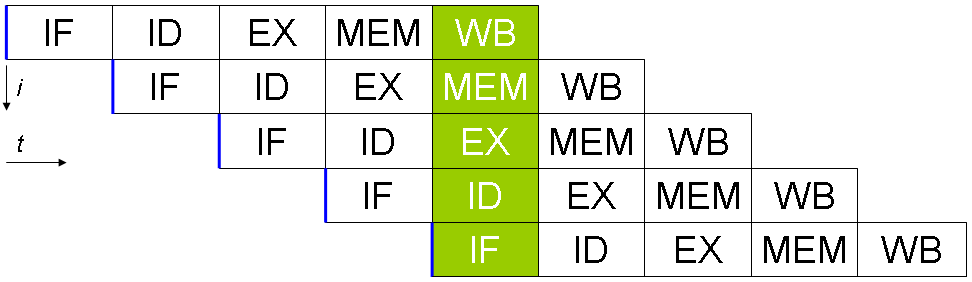
\includegraphics[width=0.8\textwidth]{img/scalar.png}
  \caption{Scalar processor}
  \label{fig:scalar}
\end{figure}

In practice however, data and control dependencies between successive instructions could cause hazards and force the pipeline to stall, causing \ac{CPI} to rise once again at values greater than one. There are mainly three types of hazards that can take place in a pipelined processor:
\begin{itemize}
  \item \textbf{Structural hazards} arise when a hardware block is needed by two or more instructions at the same point in time. For instance, if a processor features only one memory block for both instructions and data, then two different instructions executing in the fetch and memory access stages could generate a structural hazard when trying to read from memory. Such hazards can either be easily solved (e.g. separate instruction and data memory in this example) or are known and accepted by the designers, given the limited hardware available.
  \item \textbf{Data hazards} in a simple pipelined processor occur when there is a \emph{data dependence} between instructions, that is one instruction needs to read a value that provided by a previous instruction. For example, in
      \begin{verbatim}
        add    x1,x2,x3
        sub    x4,x5,x1
      \end{verbatim}
      the \texttt{sub} instruction needs the value of register \texttt{x1} in the decode stage, but the previous \texttt{add} has not yet reached the write back stage and a data hazard is generated.
  \item \textbf{Control hazards} arise in the case of conditional flow changing instructions, such as branches, that prevent following instructions to be fetched until the new direction is resolved.
\end{itemize}

The real \ac{CPI} a pipelined processor can achieve is then given by the sum of the ideal \ac{CPI} and all the delays introduced by pipeline stalls caused by hazards \cite[p.~168]{hennessy17}:
\begin{equation}\label{eq:pipe_cpi}
  \begin{split}
    \text{CPI}  & = \text{Ideal CPI} + \text{Structural stalls} + \text{Data hazard stalls} + \text{Control stalls} \\
                & = 1 + \text{Structural stalls} + \text{Data hazard stalls} + \text{Control stalls} > 1
  \end{split}
\end{equation}

Those hazards become more frequent and more expensive to manage the more pipeline stages are introduced and that is a clear example of a tradeoff between two factors of the performance equation \eqref{eq:perf}: a deeper pipeline shortens the critical path and thus reduces the clock period, but at the same time it increases the CPI. That is the reason why designers at some point had to find other architectural solutions to improve performance.

\subsection{Multiple-issue processors}
A processor featuring a single execution pipeline can only achieve a theoretical \ac{CPI} of 1, but by duplicating the pipeline to include multiple execution units more than one instruction per clock cycle could be delivered. That is the idea that lies behind \emph{multiple-issue} processors, that exploit \ac{ILP} by executing independent instructions on separate execution pipelines.

Instructions that can be issued independently to the different pipelines are selected among a so called \emph{basic block}, that is a sequence of instructions comprised between single entry and exit points (i.e. with no branches or jumps in between). Recalling the examples of the previous section, figure \ref{fig:superscalar} shows the execution scheme for a multiple issue processor.

\begin{figure}[hbtp]
  \centering
  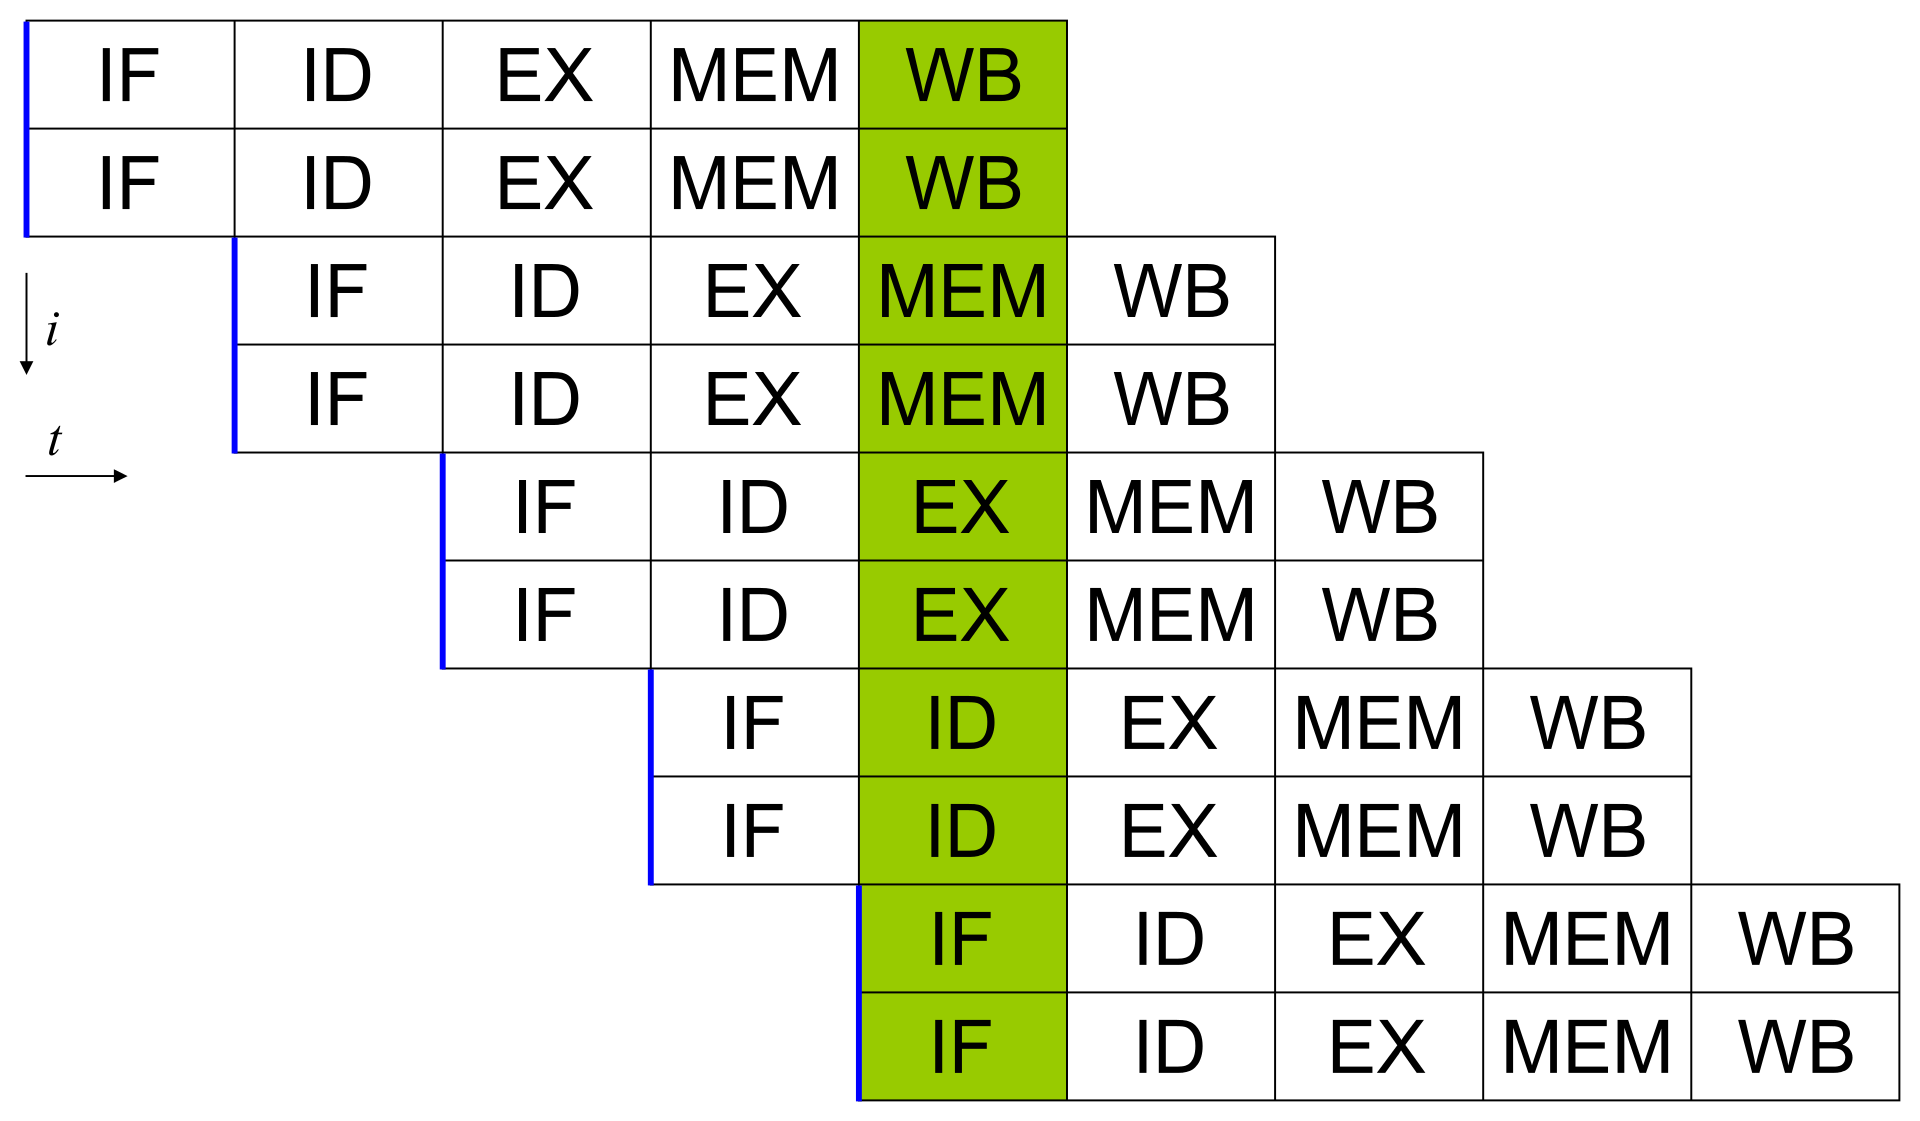
\includegraphics[width=0.8\textwidth]{img/superscalar.png}
  \caption{Multiple-issue processor with two pipelines}
  \label{fig:superscalar}
\end{figure}

Two main different approaches exist to multiple issue processors:
\begin{itemize}
  \item \textbf{\ac{VLIW}} processors, also known as \emph{static} multiple-issue, rely on software to discover \ac{ILP} chances at compile time, thus avoiding increased hardware complexity. The compiler groups instructions that can be executed in parallel in a single long packet-like instruction (hence the name \ac{VLIW}), that is then split and issued to the different execution units at run time. Despite many efforts, however, such static techniques reveal efficient only for specific applications presenting a high level of data parallelism \cite[p.~168]{hennessy17}, mainly because the compiler software needs a perfect knowledge of the underlying architecture in order to efficiently exploit \ac{ILP}.
  \item \textbf{Superscalar} processors, also known as \emph{dynamic} multiple-issue, on the other hand, rely on dedicated hardware to exploit \ac{ILP} at run time. Instructions belonging to a basic block are inserted into a \ac{WOE}, from where instruction that can run in parallel thanks to no data dependence are selected and issued to the respective following pipeline stages. This dynamic approach has been shown to work better than a static one, at the cost of a significant hardware complexity overhead.
\end{itemize}

Multiple-issue processors can achieve a \ac{CPI} lower than 1 (usually expressed at this point as \ac{IPC}, greater than 1) thanks to duplicate hardware units that also lower the impact of structural hazards, but they are nonetheless subject to data and control hazards. Instructions belonging to the same basic block are very likely to depend upon one another, as they are part of the same piece of program, and as such the amount of \ac{ILP} in contiguous instructions of a basic block is usually very small, leading to a low usage of the additional pipelines, and that is the reason why allowing multiple issues is not very useful by itself, but is almost always paired with the techniques analyzed in the next section.

\section{Dynamic scheduling}
All the processors seen in the previous sections adopted a so called \emph{static scheduling} of the pipeline, meaning that instructions are issued and executed along the pipe strictly in program order. To really extract the benefits of \ac{ILP}, however, all modern high-end processor employ a \emph{dynamically scheduled} pipeline, that can execute instructions out of order with respect to the assembled program. As an example consider the following code:
\begin{verbatim}
  add    x1,x2,x3
  sub    x5,x1,x4
  mul    x12,x18,x19
\end{verbatim}
In a classic 5-stage statically scheduled pipeline, instructions are executed in-order, and that means that the \texttt{mul} instruction cannot begin execution until the data dependence between \texttt{add} and \texttt{sub} is resolved by stalling the pipeline, as the execution takes place in program order. By using dynamic scheduling, on the other hand, if there are no structural hazards (and we can safely assume that that is the case, as the multiplier is likely to be a separate block from the \acsu{ALU}), the \texttt{mul} can be executed and maybe even completed before the \texttt{sub}. Instructions are then still issued in-order to the execution stage from the window of execution, but they can begin and complete execution \ooo.

Dynamic scheduling is almost always used in conjunction with superscalar processors, because the advantages given by the \ooo execution and the availability of multiple functional units go hand in hand. This combination offers several strengths compared to static scheduling or \ac{VLIW} processors \cite[p.~192]{hennessy17}. For instance, it allows compiled code to run in an efficient way on different microarchitectures, as the pipeline can manage itself and exploit \ac{ILP} without needing the help of the compiler. Moreover, it can handle cases where dependencies cannot be found at compile time, such as memory operations or dynamic branches. But the most important advantage of all is that an \ooo processor is able to mask the effect of unpredictable delays in the pipeline by executing later instructions without stalling. Remember that cache misses can easily take hundreds of clock cycles to resolve, which would turn into hundreds of wasted cycles in an in-order processor, but are instead taken advantage of to carry out unrelated tasks in an \ooo one.

In order to do so, the \ac{WOE} acts as a buffer between the fetch stages (called \emph{frontend}) and the execution and commit stages (called \emph{backend}), that hopefully always contains enough instructions to ensure a constant flow to the functional units, even when earlier instructions are waiting for some event. This is obviously possible only if the frontend is able to maintain a high enough bandwidth of fetched instructions to the \ac{WOE}.

\subsection{Dependencies and hazards}
Out-of-order processors are subject to all the dependencies listed in section \ref{sec:ilp}, but due to the reordering of instructions, other hazards can arise from so called \emph{name dependencies}. In this context, a useful taxonomy to categorize such hazards is defined\footnote{Structural and control hazards are not considered here, as they are the same as in an in-order processor.}. Let $D(i)$ be the \emph{domain} and $R(i)$ be the \emph{range} of instruction $i$, meaning respectively the registers or memory locations read and written by instruction $i$, and consider two instructions $i$ and $j$, with $j$ following $i$ in the program order. Then, there are three possible kinds of data hazards:
\begin{itemize}
  \item \textbf{\ac{RAW}} hazards are the only true data hazards arising from a data dependence and occur, as seen previously, when instruction $j$ is trying to read a piece of data before $i$ writes it, leading to a wrong value read by $j$, as in the following example:
      \begin{verbatim}
        add    x1,x2,x3
        sub    x4,x5,x1
      \end{verbatim}
      More formally, \ac{RAW} hazards occur if:
      \begin{equation*}
        R(i) \cap D(j) \neq \varnothing
      \end{equation*}
  \item \textbf{\ac{WAR}} hazards arise from the name dependence called \emph{anti-dependence}, that occurs when instruction $j$ writes the same location that $i$ reads, causing $i$ to read the wrong value if $j$ is executed first, as in:
      \begin{verbatim}
        add    x1,x2,x3
        mul    x2,x5,x6
      \end{verbatim}
      More formally, \ac{WAR} hazards occur if:
      \begin{equation*}
        D(i) \cap R(j) \neq \varnothing
      \end{equation*}
  \item \textbf{\ac{WAW}} hazards arise from the name dependence called \emph{output dependence}, that occurs when instructions $i$ and $j$ write their outputs on the same storage locations, leaving the final wrong value written by $i$, if $j$ is executed first, like in the following:
      \begin{verbatim}
        add    x1,x2,x3
        mul    x1,x5,x6
      \end{verbatim}
      More formally, \ac{WAW} hazards occur if:
      \begin{equation*}
        R(i) \cap R(j) \neq \varnothing
      \end{equation*}
\end{itemize}

It is hopefully clear that \ac{WAR} and \ac{WAW} hazards occur only in dynamically scheduled processors where instruction order can be rearranged and that the dependencies that cause them are called name dependencies, because it is only a matter of storage location used and not an issue with the correct outcome of the program. In the examples above, if the \texttt{mul} instruction could (temporarily) write its output on a different register, until the \texttt{add} completes, then the semantics of the program would respected and the hazards resolved without stalling. That is the idea that lies behind \emph{register renaming}, which is the technique used in \ooo processors at the decode stage to detect and solve \ac{WAR} and \ac{WAW} hazards by converting the architectural registers that instructions refer to to different physical registers hidden to the programmer and compiler.

\subsection{Scheduling techniques}
Out-of-order execution needs dedicated hardware to select instructions inside the \ac{WOE} and detect and prevent hazards. For this purpose, several schemes and algorithms exist, among which are \emph{scoreboarding} and \emph{Tomasulo's algorithm} that are described in the following.

\subsubsection{Scoreboarding}
Scoreboarding is a centralized scheduling technique first introduced in the CDC 6600 in the 60s \cite{scoreboard} and still widely used today. The algorithm provides the following stages for each instruction after the decoding:
\begin{itemize}
  \item \textbf{Issue}: instructions stall in this stage until there are no structural hazards and all the output dependencies with previously issued instructions are resolved, to avoid \ac{WAW} hazards.
  \item \textbf{Read operands}: instructions can proceed when their operands are available, resolving \ac{RAW} hazards, in an \ooo fashion.
  \item \textbf{Execute}: operands are passed to the functional units that perform the requested operations.
  \item \textbf{Write result}: the write back operation is stalled until all earlier instructions that are anti-dependent have read the previous value, resolving \ac{WAR} hazards. 
\end{itemize}

Each of these stages can take an arbitrary number of cycles, thus, in order to control the progress of all instructions, a set of three data structures is used as shown in figure \ref{fig:scoreboard}.
\begin{figure}[hbtp]
  \centering
  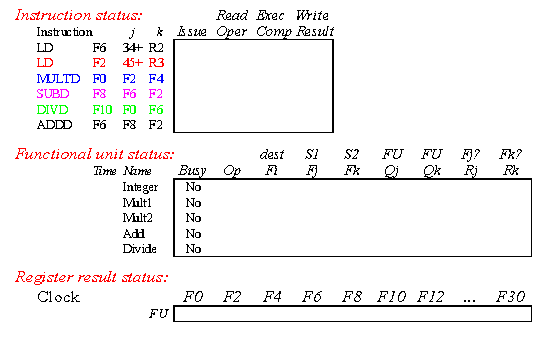
\includegraphics[width=0.8\textwidth]{img/scoreboard.pdf}
  \caption{Scoreboard structure}
  \label{fig:scoreboard}
\end{figure}
The first one is the \emph{instruction status} table, that keeps track of which of the four stages each instruction is currently in. Then, there is the \emph{functional unit status} table, which has nine fields for each functional unit, indicating if that unit is busy, what operation it has to perform, the destination register, the source operands registers, the functional units that will produce the operands and two flags indicating when those operands are ready. Finally, the \emph{register result status} table indicates for each register which functional unit will write its result to it.

The original scoreboarding algorithm did not include register renaming and so \ac{WAW} and \ac{WAR} hazards could potentially cause the pipeline to stall in the issue and write result stages respectively. For this reason, register renaming can still be implemented, but it must be carried out in the issue stage, by a dedicated renaming unit, like the one shown in figure \ref{fig:renaming}, based on the one included in the MIPS 10000.
\begin{figure}[hbtp]
  \centering
  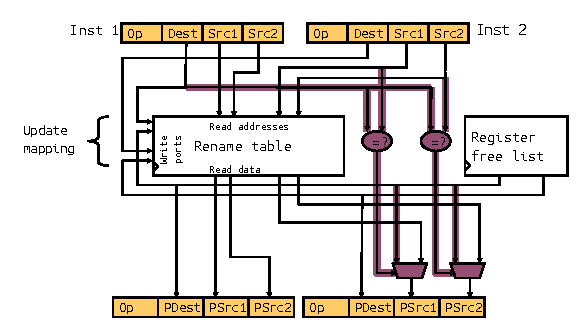
\includegraphics[width=0.9\textwidth]{img/renaming.pdf}
  \caption{Renaming unit}
  \label{fig:renaming}
\end{figure}
The \emph{rename table} keeps track of the mapping between architectural and physical registers, to maintain correct value references, while the \emph{register free list} contains the names of all available physical registers to be used for renaming. As this unit renames two instructions in parallel, it has to check for \ac{RAW} hazards between them, and in case there is one, rename the second instruction with the newly assigned physical registers to the other one. 

Using this scheme, also known as \emph{explicit} register renaming, \ac{WAW} and \ac{WAR} hazards are completely avoided as early as an instruction is decoded and issued, meaning that no further checks must be performed in the later stages of the algorithm.

\subsubsection{Tomasulo's algorithm}
Invented by Robert Tomasulo for the IBM 360/91 \ac{FPU}, this algorithm offers a different approach to dynamic scheduling, by adopting a \emph{distributed} control instead of a centralized one, as present in scoreboarding. This idea is based around the concept of \emph{reservation stations}, which are buffers placed in front of each functional unit, including load and store units, to store instruction operands. A generic architecture based on Tomasulo's approach is shown in figure \ref{fig:tomasulo}.
\begin{figure}[hbtp]
  \centering
  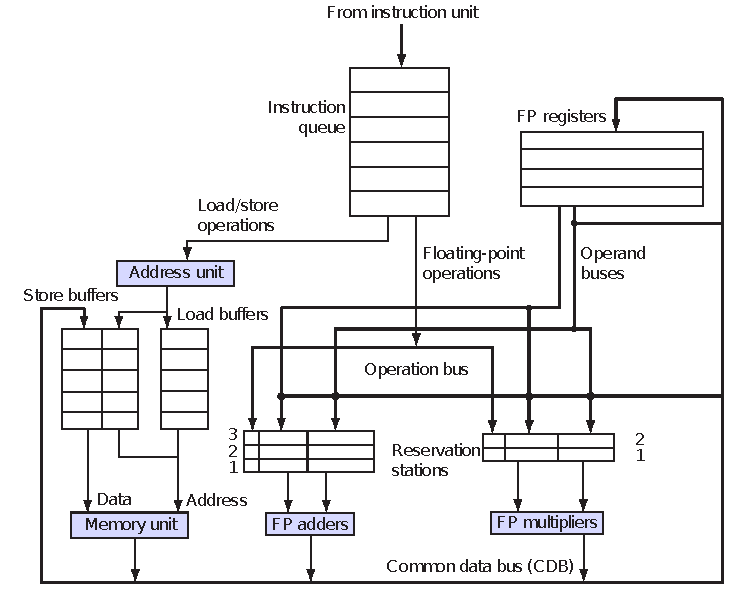
\includegraphics[width=0.9\textwidth]{img/tomasulo.pdf}
  \caption{\acs{FPU} example architecture using Tomasulo's algorithm \cite[p.~198]{hennessy17}}
  \label{fig:tomasulo}
\end{figure}

Each reservation station contains several fields providing similar information with respect to functional unit status data structure used in scoreboarding: which operation to perform, the reservation stations from which the source operands will come, the value of the operands and the busy status. The key difference with scoreboarding is, however, that the results of the functional units are broadcast to the register file as well as to all the reservation stations through a \ac{CDB}, while the scoreboarding technique only writes results to registers. This, in turn, provides the great advantage of allowing \emph{implicit} register renaming at each reservation station, because register names are discarded when an instruction is issued to a reservation station, as operands will come from another reservation station of from the \ac{CDB} as soon as they become available. Moreover, if multiple instructions are waiting on the same result, they can all be started simultaneously when such result arrives because of the presence of multiple reservation stations, while on the other hand, using scoreboarding, they would wait in turn for the register file bus to be free, possibly wasting clock cycles \cite[p.~201]{hennessy17}.

In the end, the steps that each instruction must get through are similar to the one in scoreboarding, but the actions performed are different:
\begin{itemize}
  \item \textbf{Issue}: instructions are fetched in-order from the issue queue stall in this stage until there is a matching reservation station available (no structural hazards) and then are issued to the reservation station with implicit renaming.
  \item \textbf{Execute}: the \ac{CDB} is monitored until all operands are available (avoid \ac{RAW} hazards), at which point the functional unit executes the instruction.
  \item \textbf{Write result}: as soon as an operation completes, the result is written on the \ac{CDB} and from there to the register file and reservation stations.
\end{itemize}

Tomasulo's algorithm is today used in many high-performance processors and it has been chosen also for the design of LEN5.

\section{Hardware-based speculation}
For typical \acp{ISA} around 10--20\% of instructions are branches, meaning that an average basic block will not contain more than 5 to 10 instructions. This is obviously a significant constraint, as the amount of \ac{ILP} that can be exploited in such a small set of instructions without incurring in control dependencies is quite limited. From these reason the idea of \emph{hardware-based speculation} was born, based on three principles \cite[p.~208]{hennessy17}:
\begin{itemize}
  \item Dynamic branch prediction, to fetch and issue instructions before the outcome of a branch is determined (refer to section \ref{sec:dynbp} for details).
  \item Speculative execution, to allow the execution of such instructions even if their control dependencies are not resolved yet.
  \item Dynamic scheduling, to schedule instructions crossing the boundary of a single basic block.
\end{itemize}

This represents an important improvement over mere dynamic scheduling and even branch prediction alone, because this way instructions are executed as if the guesses on the taken direction were always correct, leading to a \emph{data flow execution} of the program, where operations are executed as soon as their operands are available, irrespective of control flow.

Of course, some precautions must be taken in order to handle the situation when the speculated flow was predicted incorrectly, as to restore the original state of the processor and proceed down the right path. For this reason, an additional stage after the write result must be inserted in order to decouple the production of a result by a functional unit and the actual irreversible update of the register file and data memory, that can take place only when an instruction is no longer speculative. This last step is called \emph{instruction commit} and must always be performed in-order.

\subsection{\acl{ROB}}
In both scoreboarding and Tomasulo's approach, instruction commit can be handled using a dedicated hardware structure called \ac{ROB}. As the name implies, the \ac{ROB} acts as a buffer between the functional unit outputs and the register file and memory, storing speculative results until the speculation is resolved and thus effectively increasing the number of registers available, similarly to reservation stations. A general scheme of an architecture using the \ac{ROB} is shown in figure \ref{fig:robpipe}, highlighting which parts of the pipeline are in-order and which \ooo.
\begin{figure}[hbtp]
  \centering
  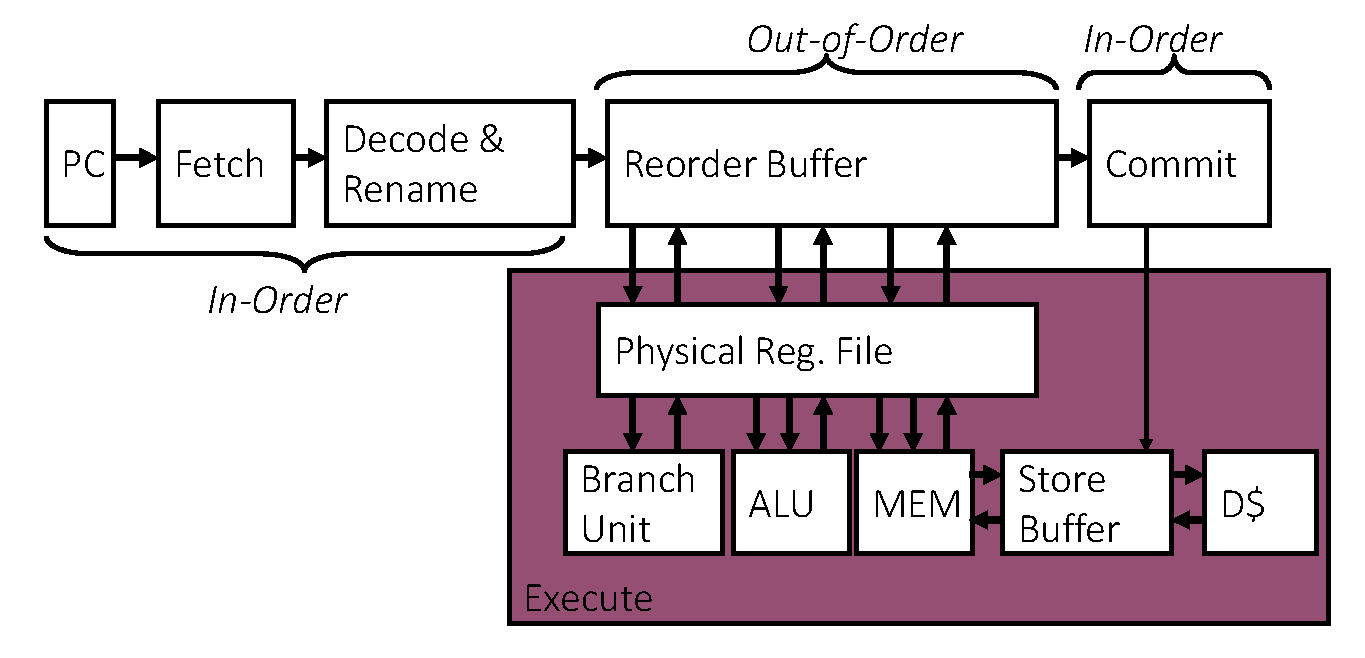
\includegraphics[width=0.8\textwidth]{img/robpipe.pdf}
  \caption{An \ooo pipeline featuring register renaming and \acs{ROB}}
  \label{fig:robpipe}
\end{figure}

\subsubsection{\acs{ROB} with Tomasulo's algorithm}
As stated above, the \ac{ROB} extends the number of available registers and thus provides renaming on its own by substituting the register file before instruction commit. Moreover, alongside the reservation stations and the \ac{CDB}, the \ac{ROB} serves as another source of operands, as figure \ref{fig:robtomasulo} shows. Finally, for its intrinsic nature, the \ac{ROB} also serves almost the same purpose of the store buffer as a reservation station before the data memory.
\begin{figure}[hbtp]
  \centering
  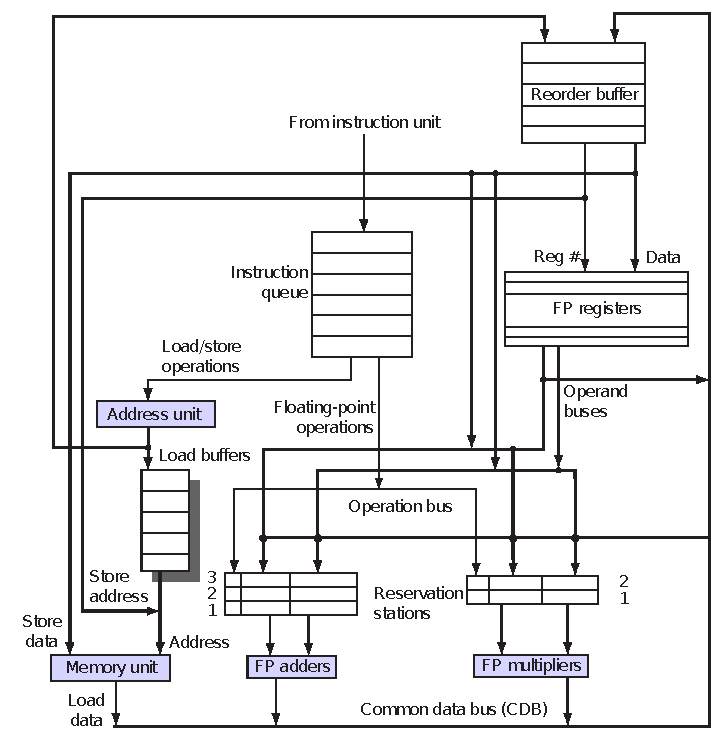
\includegraphics[width=0.8\textwidth]{img/robtomasulo.pdf}
  \caption{\acs{FPU} example architecture using Tomasulo's algorithm and \acs{ROB} \cite[p.~210]{hennessy17}}
  \label{fig:robtomasulo}
\end{figure}

In terms of algorithm steps, what changes is that during execution the results are broadcast on the \ac{CDB} and to the \ac{ROB} instead of to the register file. In addition, during the added step of instruction commit, an instruction is removed when it reaches the head of the \ac{ROB} (which acts as a circular buffer) and, if it is a branch with a wrong prediction to reach the commit stage, then the \ac{ROB} gets flushed and execution resumes at the correct target of the branch.

\section{Summary of \acs{ILP} techniques}
To summarize this overview of multiple-issue processors and techniques to exploit \ac{ILP}, table \ref{tab:multissue} provides all the important differences at a glance.
\begin{table}[hbtp]
  \centering
  \rowcolors{1}{}{gray!10}
  \makebox[\textwidth][c]{
    \begin{tabular}{p{\dimexpr 0.16\linewidth}
                    p{\dimexpr 0.13\linewidth}
                    p{\dimexpr 0.13\linewidth}
                    p{\dimexpr 0.14\linewidth}
                    >{\raggedright}p{\dimexpr 0.18\linewidth}
                    >{\raggedright\arraybackslash}p{\dimexpr 0.22\linewidth}}
      \toprule
      \textbf{Name} & \textbf{Issue structure} & \textbf{Hazard detection} & \textbf{Scheduling} & \textbf{Relevant features} & \textbf{Examples} \\ \hline
      Superscalar (static) & Dynamic & Hardware & Static & In-order    execution & Embedded MIPS and ARM cores \\
      Superscalar (dynamic) & Dynamic & Hardware & Dynamic & Out-of-order execution, but no speculation & None \\
      Superscalar (speculative) & Dynamic & Hardware & Dynamic & Out-of-order execution and speculation & Intel Core i3, i5, i7, AMD Ryzen \\
      \ac{VLIW} & Static & Software & Static & Hazards detected by the compiler & Signal processors like the TI C6x \\
      \bottomrule
    \end{tabular}
  }
  \caption{Summary table of multiple-issue approaches \cite[p.~219]{hennessy17}}
  \label{tab:multissue}
\end{table}
\todo{Ariane e BOOM??}
\chapter{LEN5 frontend}
\section{General block diagram}
\begin{figure}[hbt]
  \centering
  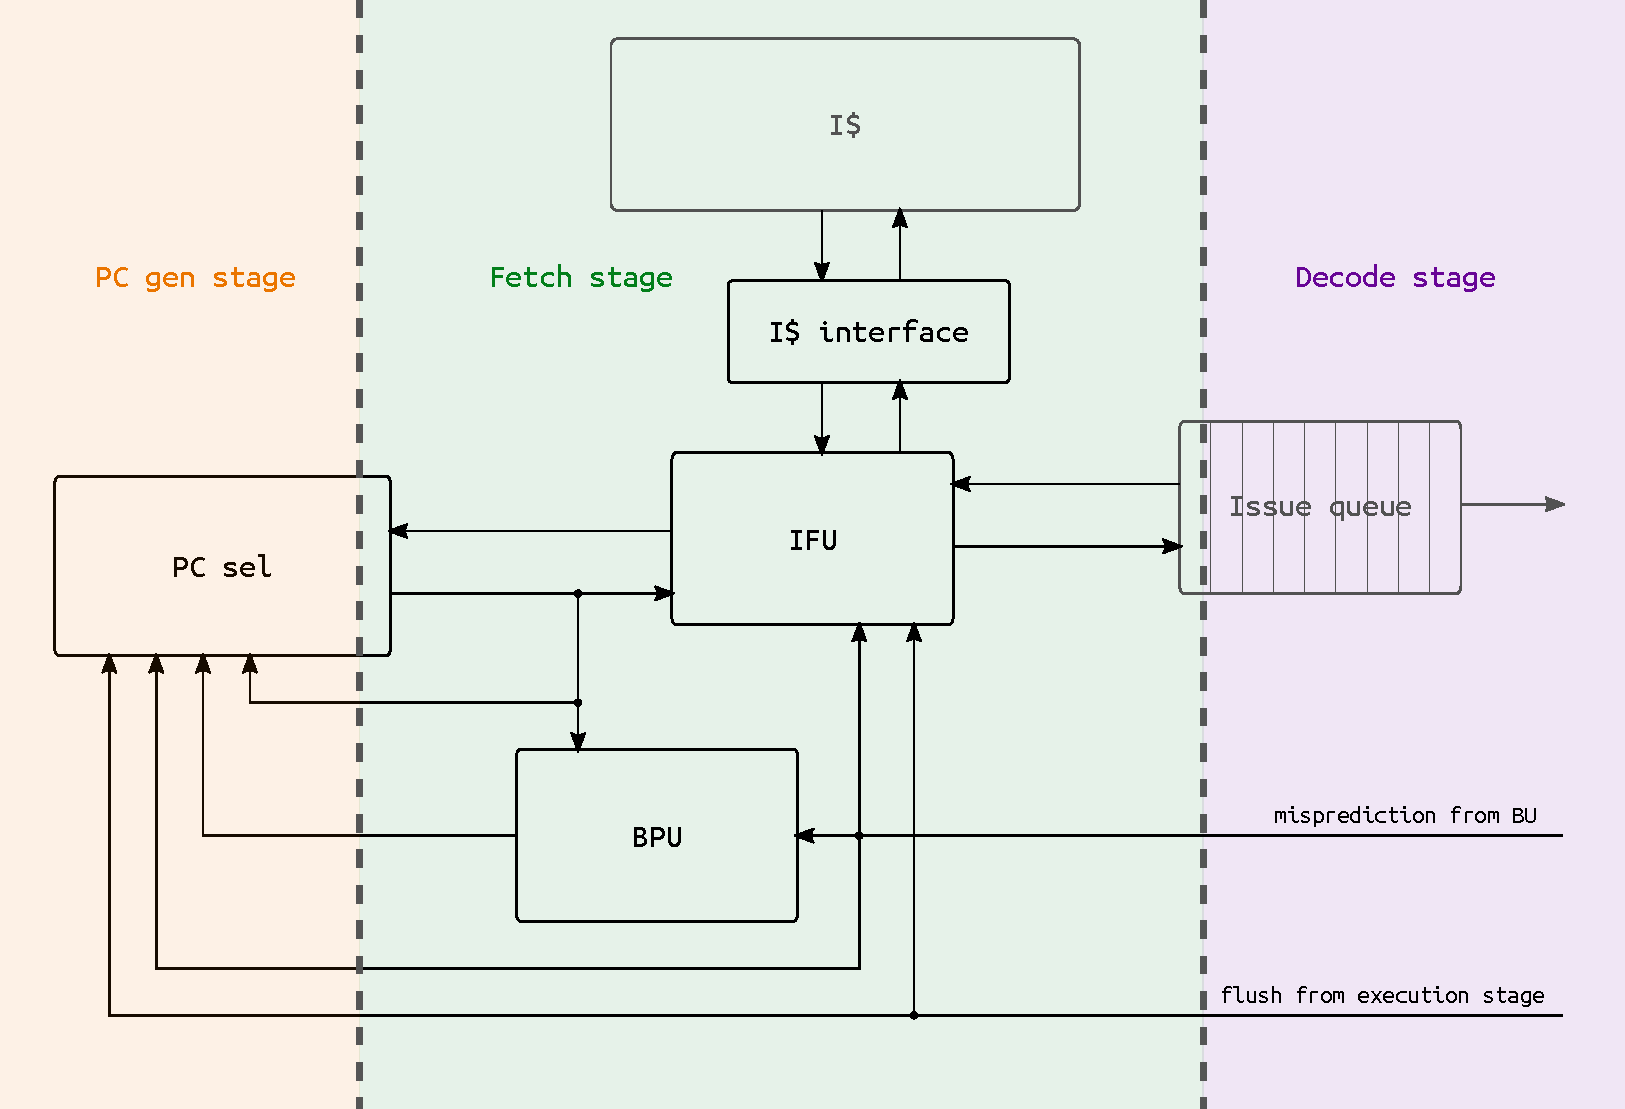
\includegraphics[width=\textwidth]{img/frontend.pdf}
  \caption{LEN5 frontend}
  \label{fig:frontend}
\end{figure}
\Cref{fig:frontend} shows a top-level block diagram of the LEN5 frontend, with the modules that were developed and that will be described in the following sections shown in solid black color. Gray blocks are instead the ones the frontend interfaces with, that are the instruction cache, or equivalently the memory management unit, and the issue queue.

The frontend is composed of two pipeline stages, namely the \emph{\ac{PC} generation} and the \emph{fetch} stages. \Cref{fig:frontend} also shows the \emph{decode} stage, where the issue queue is found. The latter is basically a \acs{FIFO} that serves as a buffer interface between the frontend and the backend of the processor by storing a queue of instructions to be issued to the later stages of the pipeline.

\subsection{\acs{PC} gen stage}
In the \ac{PC} generation (\ac{PC} gen) stage, the next \ac{PC} is selected among a number of different options by the \ac{PC} sel block, using a predefined priority, and is then written on the output register of the stage. This register also serves as the pipeline register between the two stages, and that is why \cref{fig:frontend} shows a dashed gray line crossing the \ac{PC} sel block. 

The selection of the new \ac{PC} is carried out by a network of combinational logic, so that this stage always takes exactly one clock cycle.

\subsection{Fetch stage}
In the fetch stage, the \ac{PC} is used by the \acf{IFU} to select and possibly read from memory the next instruction to be pushed to the issue queue. At the same time, the \acf{BPU} uses the current address to predict the next direction in case of branch and passes such information back to the \ac{PC} gen stage. Memory accesses are performed through the instruction cache interface which manages the control signals to the instruction cache. 

The latency of this stage is at least two clock cycles (see \cref{sec:ifu}); in a normal steady state the \ac{IFU} can provide a throughput of one instruction each clock cycle to the issue queue, but in case of cache miss the number of cycles to resolve the stall can grow significantly, so the latency cannot be determined in advance. The issue queue is there exactly to provide some elasticity to the pipeline, by buffering already fetched instructions, masking at least in part this unpredictable latency.

\subsection{Handshake signals}\label{sec:handshake}
The communication between each stage is always bidirectional, because in case of a stall, caused for instance by a cache miss, by a full issue queue or by some other exceptional behavior down the pipeline, the \ac{PC} generation process must be interrupted along with the fetch. In order to do so, a handshake process handles the communication between each stage as well as between the instruction cache interface and the actual cache.

This handshake mechanism is based on the {\smaller AXI} valid/ready protocol described below, even if it is not compliant with all the {\smaller AXI} specifications.

In each communication the source of data generates a \emph{valid} signal to indicate that the information is available, while the destination generates a \emph{ready} signal to indicate that it can accept such information \cite[p.~A3-41]{axi}. The handshake takes place and the information is successfully exchanged only at the rising clock edge when both valid and ready are asserted. For example, in \cref{fig:axi}, the handshake happens at the third rising edge of the clock.
\begin{figure}[hbt]
  \centering
  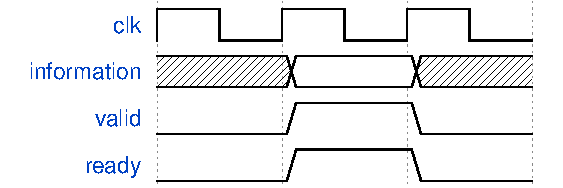
\includegraphics{img/axi.pdf}
  \caption{AXI handshake protocol}
  \label{fig:axi}
\end{figure}

When a source has information available (\cref{fig:axi_valid_ready}), it must assert valid and then wait until the corresponding ready is produced. It cannot wait for the ready before asserting valid.
\begin{figure}[hbt]
  \centering
  \subfloat[Valid before ready]{
    \label{fig:axi_valid_ready}
    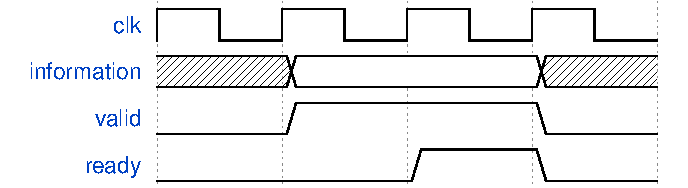
\includegraphics{img/axi_valid_ready.pdf}} \\
  \subfloat[Ready before valid]{
    \label{fig:axi_ready_valid}
    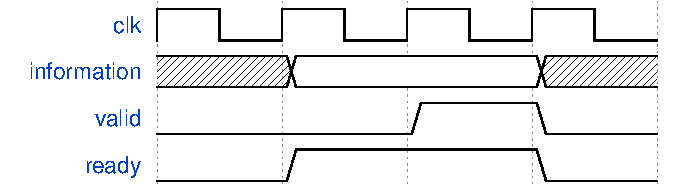
\includegraphics{img/axi_ready_valid.pdf}}
  \caption{Possible handshake timings}
  \label{fig:axi_timings}
\end{figure}
On the other hand (\cref{fig:axi_ready_valid}), a destination is allowed to wait for its valid before asserting ready and it can also deassert ready before a corresponding valid arrives.

\section{\acs{PC} gen stage}
The selection of the next \ac{PC} is based on the following list of priorities, from highest to lowest:
\begin{enumerate}
  \item \textbf{Exception}: if an exception occurs, the \ac{PC} gen stage will receive the next starting address as the base address present in the vector table provided by the {\smaller CSR} unit.
  \item \textbf{Misprediction}: if a resolved branch is discovered to have been mispredicted, then the \ac{PC} gen stage resumes execution from the correct target if the branch was actually taken, or from the next sequential address from the branch \ac{PC} if it was actually not taken.
  \item \textbf{Branch prediction}: if the \ac{BPU} predicts a taken branch for the current \ac{PC} then it provides this stage with the predicted target address (see \cref{sec:btb}), which will be fetched at the next cycle, thus allowing for zero penalty branches when predicted correctly.
  \item \textbf{Default assignment}: if none of the conditions before occur, then the next \ac{PC} is selected as usual as the next sequential address, which corresponds to the current \ac{PC}+4 for word-aligned 32-bit instructions.
\end{enumerate}

\begin{figure}[hbt]
  \centering
  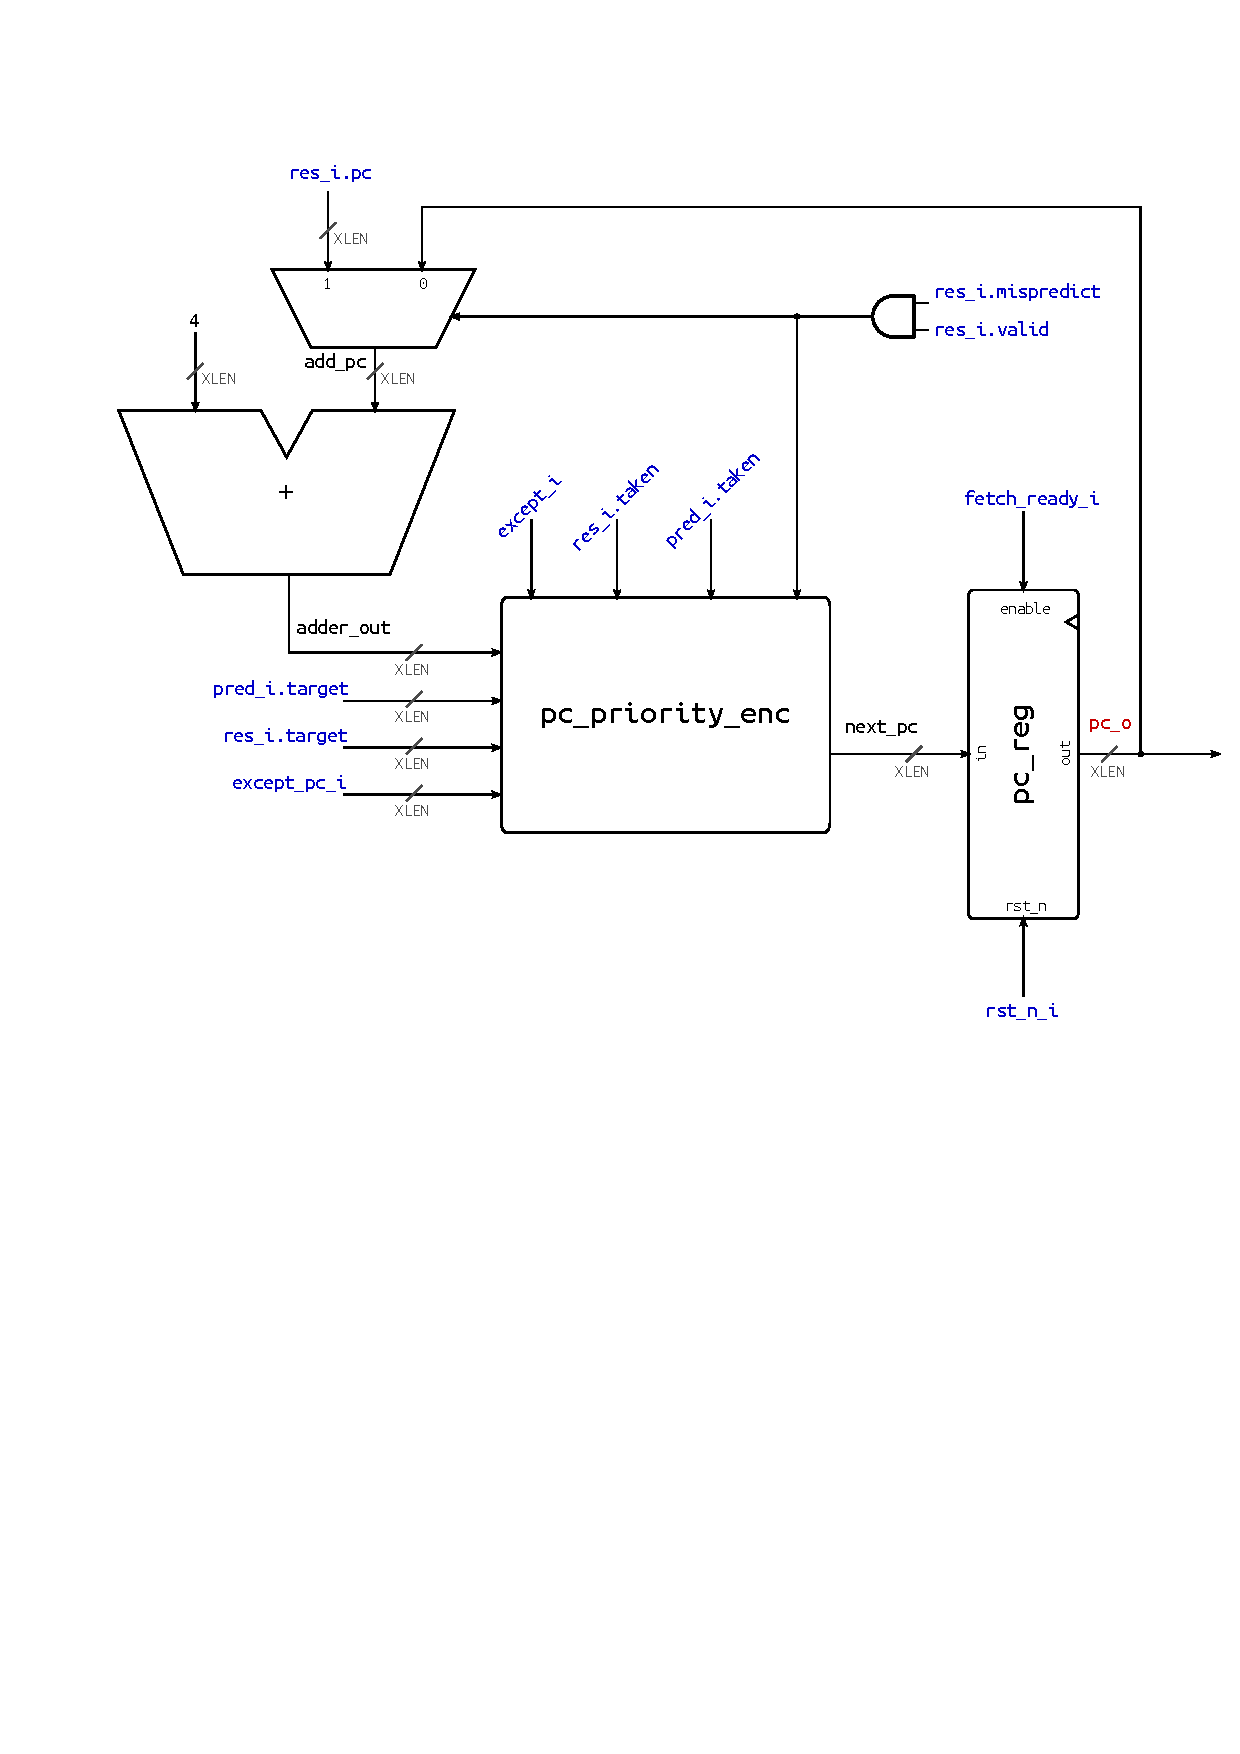
\includegraphics[width=\textwidth]{img/pc_gen_stage.pdf}
  \caption{\acs{PC} gen stage diagram}
  \label{fig:pc_gen_stage}
\end{figure}
\Cref{fig:pc_gen_stage} shows the diagram of this stage. This and all the following diagrams in this document are color coded so that input signals are in {\color{input_blue}{blue}}, output signals are in {\color{output_red}{red}}, internal signals in black and bit widths are in {\color{width_gray}{gray}}.

The heart of the \ac{PC} gen stage is the \texttt{pc\_priority\_enc} block, which is an encoder that takes as inputs all the status signals indicating a behavior different from the default and all the corresponding potential next \acp{PC}. In behavioral SystemVerilog (\cref{code:priorityenc}) it is described as a if-then-else chain, which gets synthesized as a list of cascading multiplexers implementing the desired priority\footnote{As opposed to the description using a case statement, which leads to a single parallel mux, with no priority encoded.}.
\begin{lstlisting}[
  language=Verilog,
  caption={\texttt{pc\_priority\_enc} description},
  captionpos=b,
  label=code:priorityenc
]
  always_comb begin: pc_priority_enc
    if (except_i) begin
      next_pc = except_pc_i;
    end else if (res_valid_i && res_mispredict_i) begin
      if (res_taken_i) begin
        next_pc = res_target_i;
      end else begin
        next_pc = adder_out;
      end
    end else if (pred_taken_i) begin
      next_pc = pred_target_i;
    end else begin
      next_pc = adder_out;
    end
  end: pc_priority_enc
\end{lstlisting}

In order to save resources, a single adder is used to generate both the next sequential address and the next \ac{PC} after a mispredicted not taken branch. A multiplexer driven by the misprediction signals is used to select the right operand.

The final selected next \ac{PC} is fed into the \texttt{pc\_reg} output register for the later stages. The enable of this register is controlled by the signal \texttt{fetch\_ready\_i} which comes from the fetch stage and disables the \ac{PC} generation if a stall occurs. This is part of the handshake mechanism described in \cref{sec:handshake}, even if there is no \emph{valid} signal from the \ac{PC} gen stage, as it is redundant due to the fact that a valid new \ac{PC} is always present at the output register.

\section{Instruction cache interface}
\todo{Talk about FSM coding style}
\begin{figure}[hbt]
  \centering
  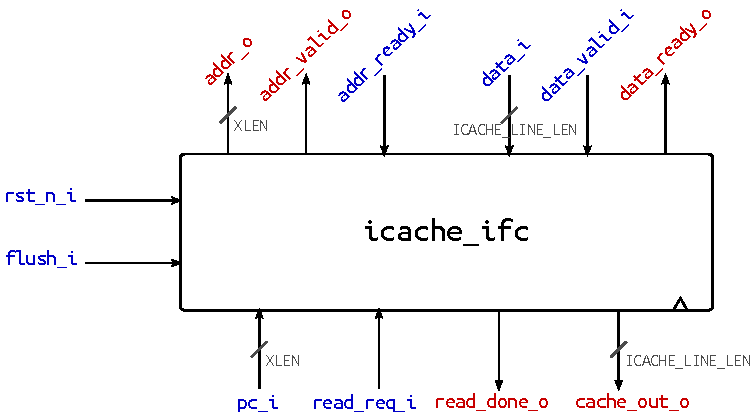
\includegraphics{img/icache_ifc-top.pdf}
  \caption{Instruction cache interface module ports}
  \label{fig:icache_ifc-top}
\end{figure}
The instruction cache interface (\cref{fig:icache_ifc-top}) is responsible for translating the fetch requests coming from the \ac{IFU} into compliant valid/ready handshake signals for both address and data to the instruction cache. This unit basically provides two main benefits. First, it simplifies the control of the \ac{IFU}, by delegating the handshake process. Second, and more important, it provides an additional separation layer between the core frontend and the instruction cache with modularity in mind so that, should the cache block be modified, only this interface block needs to be updated, while the signals coming from the \ac{IFU} module would remain unchanged.

\subsection{Datapath}
\begin{figure}[hbt]
  \centering
  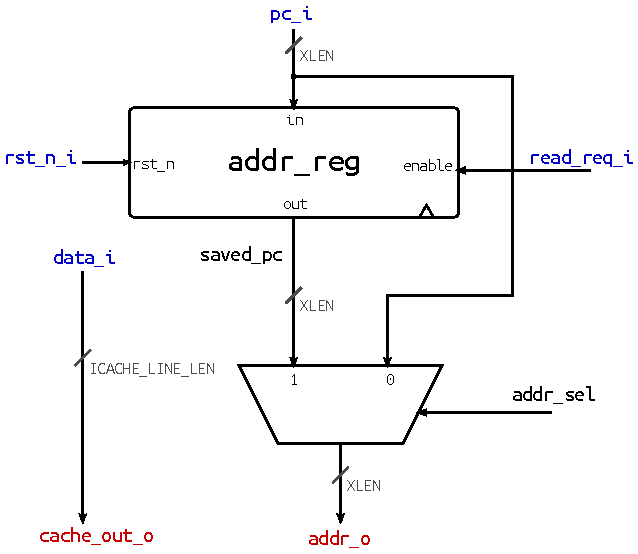
\includegraphics{img/icache_ifc.pdf}
  \caption{Instruction cache interface datapath}
  \label{fig:icache_ifc}
\end{figure}
For what concerns data signals, the line received from the is directly connected with the \texttt{cache\_out} output, as the instruction cache is responsible for keeping its output valid until the handshake occurs. On the other hand, no assumption can be done on the timing of the input address other than the fact that it will be valid in the same cycle when \texttt{read\_req} is asserted. For this reason, given the possibility for the \ac{PC} to change at the following cycle, the requested address must be retained inside the interface by means of a register, as shown in \cref{fig:icache_ifc}. The multiplexer selects the input address if the cache is ready to receive the address in the cycle the request is sent, otherwise it selects the registered address in the following cycles.

\subsection{Control \acs{FSM} and timing}
\begin{figure}[hbt]
  \centering
  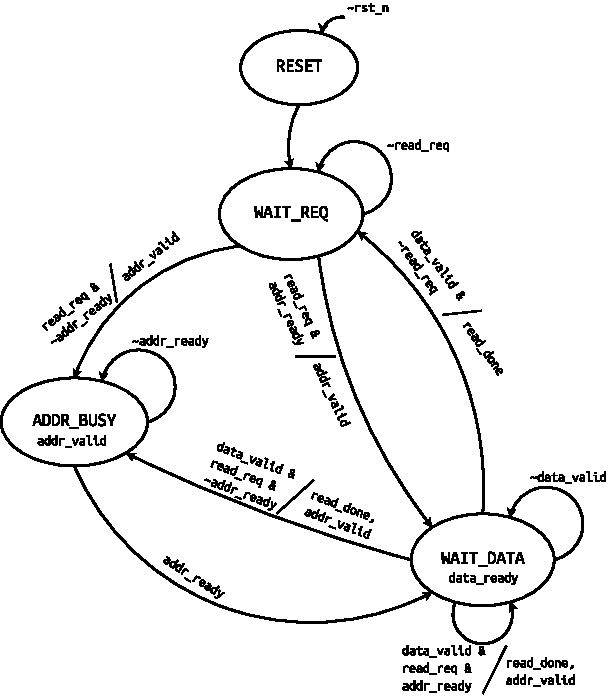
\includegraphics[scale=.8]{img/icache_ifc_fsm.pdf}
  \caption{Instruction cache interface \acs{FSM}}
  \label{fig:icache_ifc_fsm}
\end{figure}
The control unit of this block is a simple Mealy \acs{FSM} (\cref{fig:icache_ifc_fsm}) that after reset waits for a read request from the \ac{IFU}, then checks if the instruction cache is ready to receive an address and finally waits for a valid cache line to be read.

\begin{figure}[hbt]
  \centering
  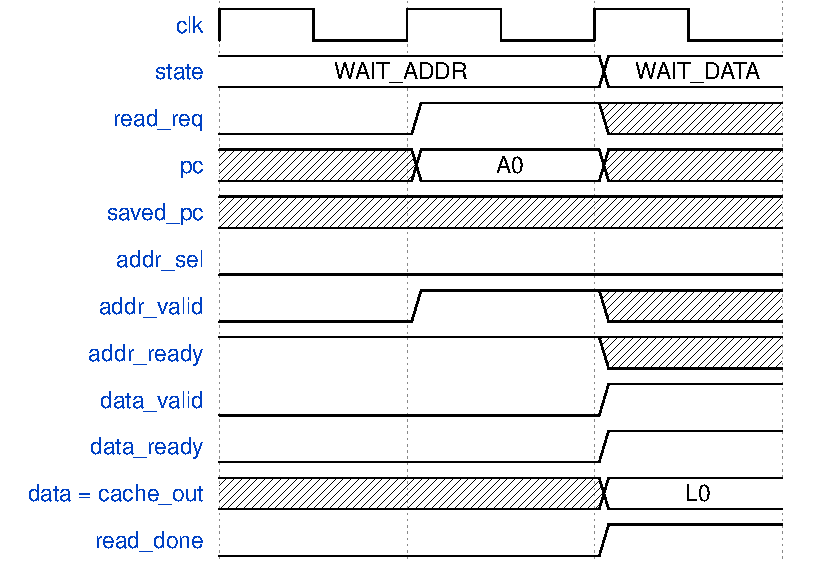
\includegraphics{img/cache01.pdf}
  \caption{Normal cache read}
  \label{fig:cache01}
\end{figure}
\Cref{fig:cache01} shows a normal cache read, where the instruction cache is immediately ready to receive an address which hits and produces the requested data at the next clock cycle. From this timing diagram it is also clear why a Mealy \acs{FSM} is needed: the signal \texttt{addr\_valid} needs to be asserted combinationally in the same clock cycle in which \texttt{read\_req} arrives, so that the address handshake can take place immediately. Otherwise, with a Moore machine, one clock cycle would be wasted at each request, rendering impossible to sustain one instruction per clock cycle fetch. Another possibility would have been not to include such signal as a Mealy output of the machine and instead connect it with a wire outside the \acs{FSM}, which would lead to the same exact result, but was deemed as less readable.

\begin{figure}[hbt]
  \centering
  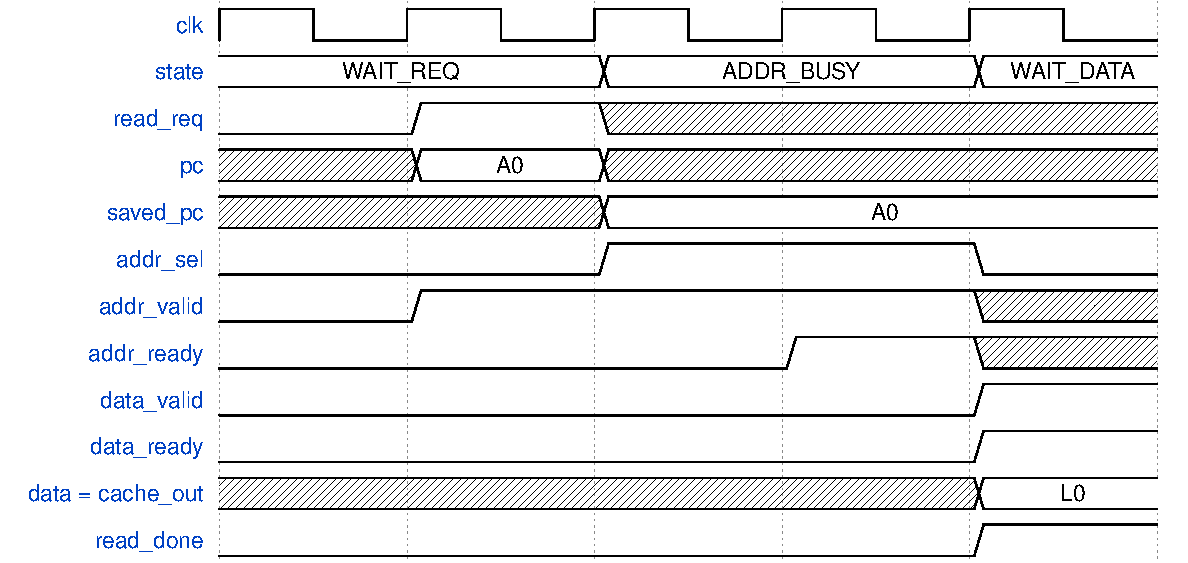
\includegraphics[width=\textwidth]{img/cache02.pdf}
  \caption{Cache not ready on address}
  \label{fig:cache02}
\end{figure}
\Cref{fig:cache02} shows another possibility when the instruction cache is not ready to receive an address at the time when a request arrives. In this case the \acs{FSM} waits until the cache become ready in the \texttt{ADDR\_BUSY} state. The state machine could just as well wait in the \texttt{WAIT\_ADDR} state, but the additional state was introduced for robustness with \texttt{addr\_valid} as a Moore output, so that this way there is no need for the \texttt{read\_req} signal to stay active until the cache is ready. This is another point in favor of a Mealy \acs{FSM} instead of the connection of combinational outputs externally. Moreover, if the \acs{FSM} loops in this waiting state, the registered address is selected for the handshake, as the original program counter could have changed by that point. 

\begin{figure}[hbt]
  \centering
  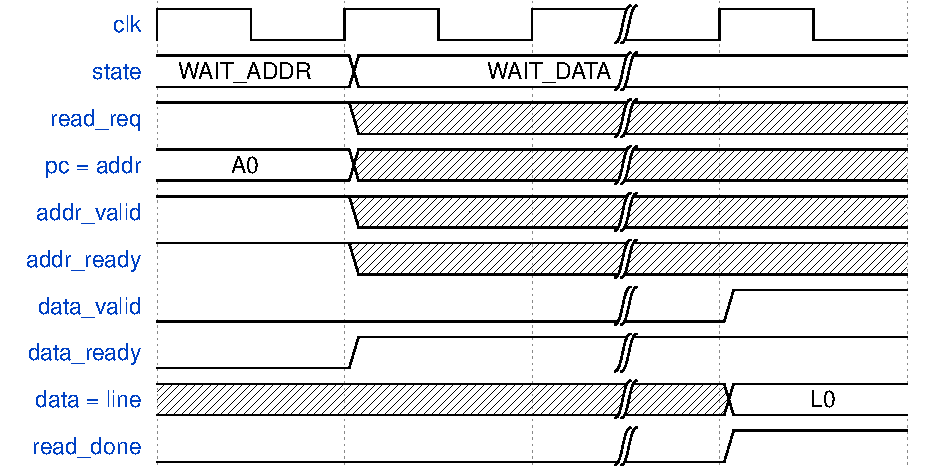
\includegraphics[width=\textwidth]{img/cache03.pdf}
  \caption{Cache miss}
  \label{fig:cache03}
\end{figure}
Finally, \cref{fig:cache03} shows the case of a cache miss, in which the \acs{FSM} waits while keeping \texttt{data\_ready} asserted. This state could potentially last for many clock cycles.

\section{\acf{IFU}}\label{sec:ifu}
\begin{figure}[hbt]
  \centering
  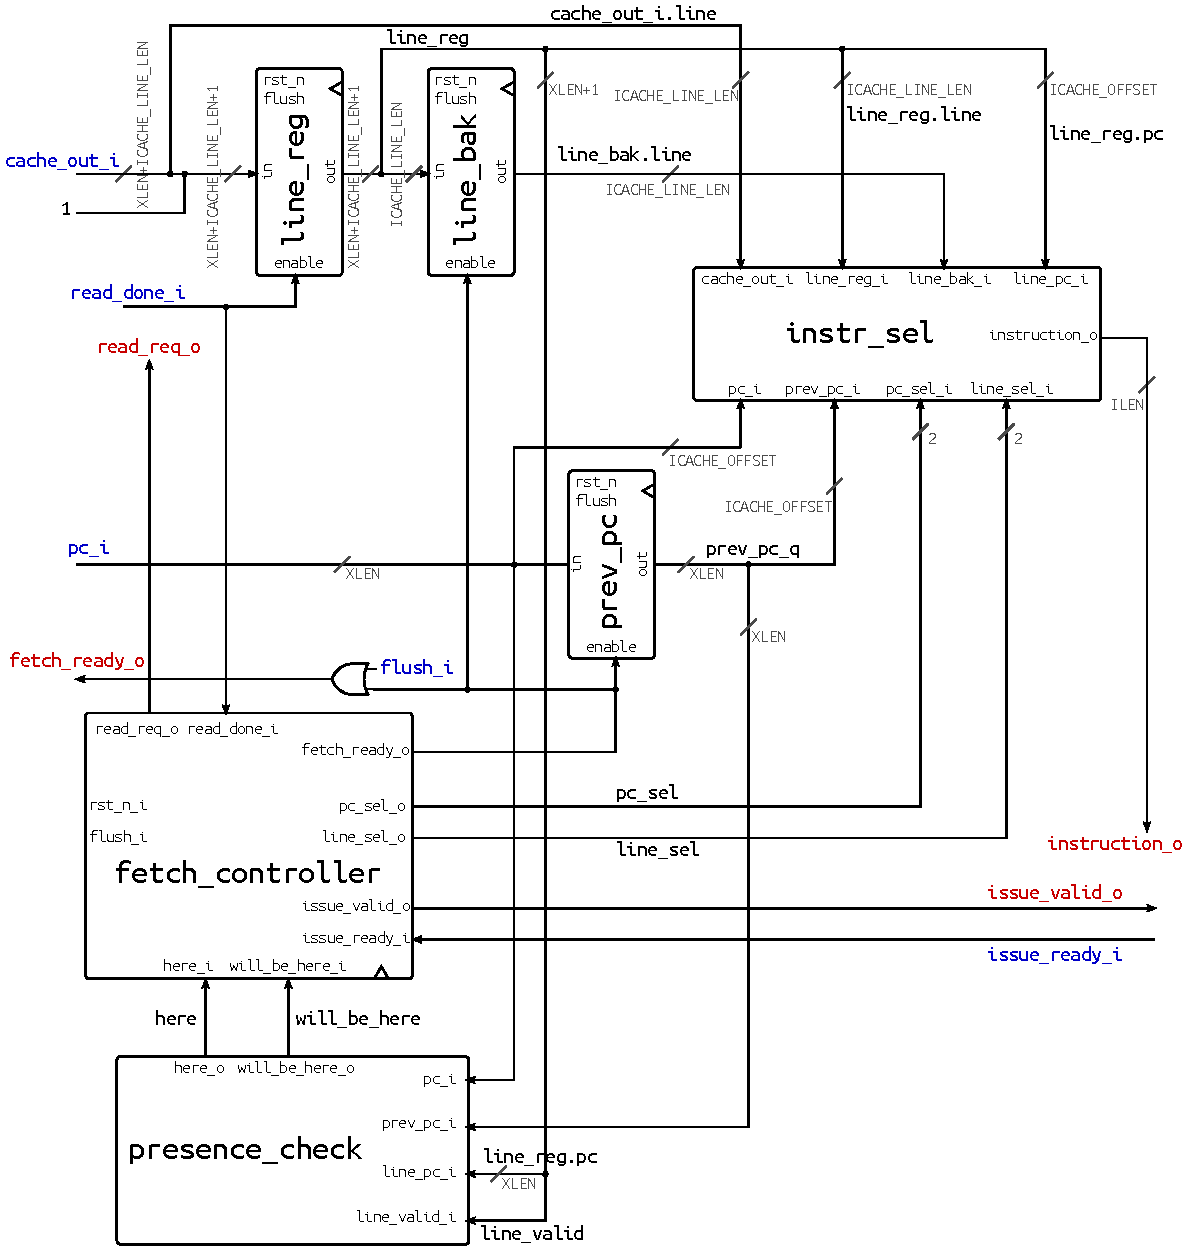
\includegraphics[width=\textwidth]{img/ifu.pdf}
  \caption[\acs{IFU} diagram]{\acs{IFU} diagram (inputs \texttt{rst\_n\_i} and \texttt{flush\_i} are shown as module port but are not connected with wires to avoid further clutter in the diagram, apart from the output OR gate)}
  \label{fig:ifu}
\end{figure}
\Cref{fig:ifu} shows the top level diagram of the \ac{IFU}, which has the ability to fetch instructions from thee different locations. The first is the direct output of the instruction cache, from which instructions are taken in case of a memory access. Then, when a cache line containing multiple instructions is read, it is saved into a \emph{line register} along with a valid bit that indicates that such line is valid. Consecutive instructions belonging to the same cache line are then fetched from this register, thus reducing the total number of cache requests. Finally, this line register is in turn saved into a \emph{line backup register} every time that a fetch takes place (i.e. the register is not updated during a stall). This additional location is used every time that the current \ac{PC} requires a cache access, but the next address refers to an instruction that was present in the previously saved cache line. Without a backup, the line register would be overwritten by the line fetched at the current \ac{PC} and so the next address would require a new cache read. Using an additional register, on the other hand, allows the \ac{IFU} to read the next instruction from the previous line. Evidently, this reasoning could be iterated to account for the second-oldest, third-oldest, etc. saved cache line, leading to a longer \acs{FIFO} of line registers among which to select the current instruction. This is definitely a possible improvement, but including more than two registers was judged out of the scope of the frontend. An actual improvement should on the other hand come from the memory system, that could for instance include a \emph{trace cache}, to account for subsequent instructions frequently fetched from different cache lines. Should such a feature be included, no other modifications would be needed on the \ac{IFU} end.

Two blocks, namely the \emph{presence checker} and the \emph{instruction selector} are responsible of informing the fetch controller if the current \ac{PC} points to an instruction already present in a saved line and of choosing the right source and the right instruction in the cache line respectively. The fetch controller itself is responsible of the orchestration of all the operations carried out inside the \ac{IFU} and of interfacing with the instruction cache interface as well as the \ac{PC} gen stage before and the issue queue after.

At the startup of the processor, the first fetch address will be the defined boot address which it is safe to assume that is going to need a cache access, as no line has been read and saved yet in the line register. This means that, even in the best case scenario (i.e. cache hit), the first instruction will be pushed to the issue queue one clock cycle after the corresponding \ac{PC} has entered the fetch stage, leading to a latency of a total of two clock cycles. In order to maintain the throughput of one instruction per clock, however, the \ac{PC} generation process must go on before knowing if the cache will hit or miss and that means that the first \ac{PC} must be saved in a \emph{previous \ac{PC} register} in order to push the correct instruction to the queue at the next cycle. In other words, at each clock cycle, the \ac{IFU} is simultaneously checking whether the current \ac{PC} refers to a saved instruction or if a cache access is needed and pushing the previous instruction to the issue queue. Actually, if the current instruction is already present in a line register, then it could be potentially moved to the queue in the same cycle as no cache latency must be accounted for. This, however, would complicate significantly the timing of this unit, as the latency would be variable according to the need of a cache read or not. For this reason, it has been chosen to maintain a one-cycle latency for every instruction, meaning that each instruction pushed to the queue corresponds to the \ac{PC} of the previous cycle. This is effectively an additional pipeline stage, introduced to account for the minimum cache latency and not to reduce the critical path.

Finally, in case of an exceptional behavior or a branch misprediction, the \ac{IFU} must be flushed and all pending cache requests aborted, in order to resume the process at the next cycle when the new starting \ac{PC} will be provided by the \ac{PC} gen stage. In order to do so, a \texttt{flush} signal that comes from the later execution stages or from the top-level control is propagated to all the sequential elements of the \ac{IFU}. This acts as a synchronous reset for all the registers and reverts back all the \acsp{FSM} to their startup state \cite{resets}, by acting directly on the state register. For this latter case, the effect is the same of having a check on the flush signal in each state, but leaving it as an external signal similar to the initial reset simplifies significantly the state diagram and helps readability.

\subsection{Presence checker}
\begin{figure}[hbt]
  \centering
  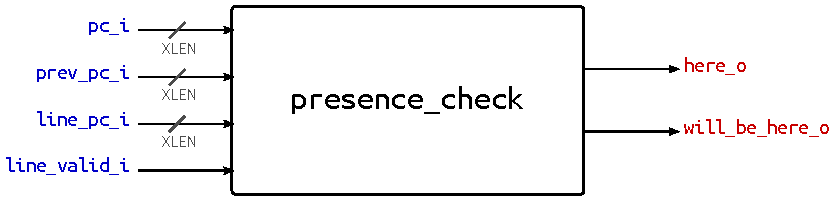
\includegraphics{img/presence_check-top.pdf}
  \caption{Presence checker module ports}
  \label{fig:presence_check-top}
\end{figure}
\begin{figure}[hbt]
  \centering
  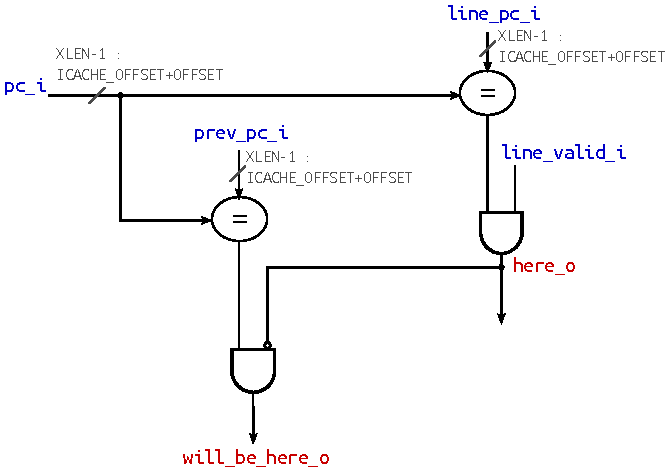
\includegraphics{img/presence_check.pdf}
  \caption{Presence checker combinational network}
  \label{fig:presence_check}
\end{figure}
The presence checker block (see \cref{fig:presence_check-top,fig:presence_check}) features a simple combinational network that performs two checks in parallel to determine the need of a new cache access by the \ac{IFU}, in particular:
\begin{itemize}
  \item If the current address refers to an instruction present in the line register and the saved line is valid, then the \texttt{here} signal indicates that no new cache read is needed and that the instruction is to be selected inside the line register.
  \item If the current address refers to an instruction in the same cache line as the previous address, then either that line is already present in the line register, or it will be the next line read from the cache and so it will be saved as soon as the read completes. In this case a \texttt{will\_be\_here} signal tells the \ac{IFU} not to request the same line twice to the memory. 
\end{itemize}
If none of these signals are asserted, then a new cache request is sent to the interface.

All the instructions belonging to the same cache line have the same most significant parts of the addresses, namely only the $N$ \acsp{LSB} differ, where:
\begin{equation*}
  N = \lceil \log_2(\text{Instructions/cache line}) \rceil + 
      \lceil \log_2(\text{Bytes/instruction}) \rceil
\end{equation*}
So, to check whether two instructions belong to the same line, a comparison between the $64-N$ (or more generally $\texttt{XLEN}-N$, where \texttt{XLEN} is the parallelism of the processor) most significant bits of their addresses is sufficient. That is what the presence checker does as shown in \cref{fig:presence_check}.

\subsection{Instruction selector}
\begin{figure}[hbt]
  \centering
  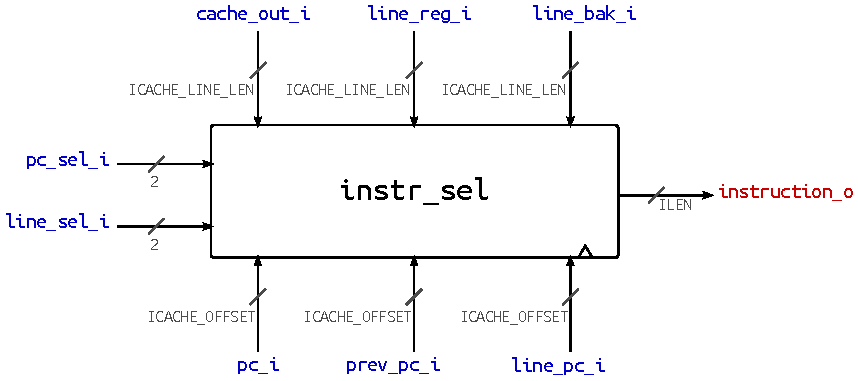
\includegraphics{img/instr_sel-top.pdf}
  \caption{Instruction selector module ports}
  \label{fig:instr_sel-top}
\end{figure}
\begin{figure}[hbt]
  %\hspace*{-1.5cm}
  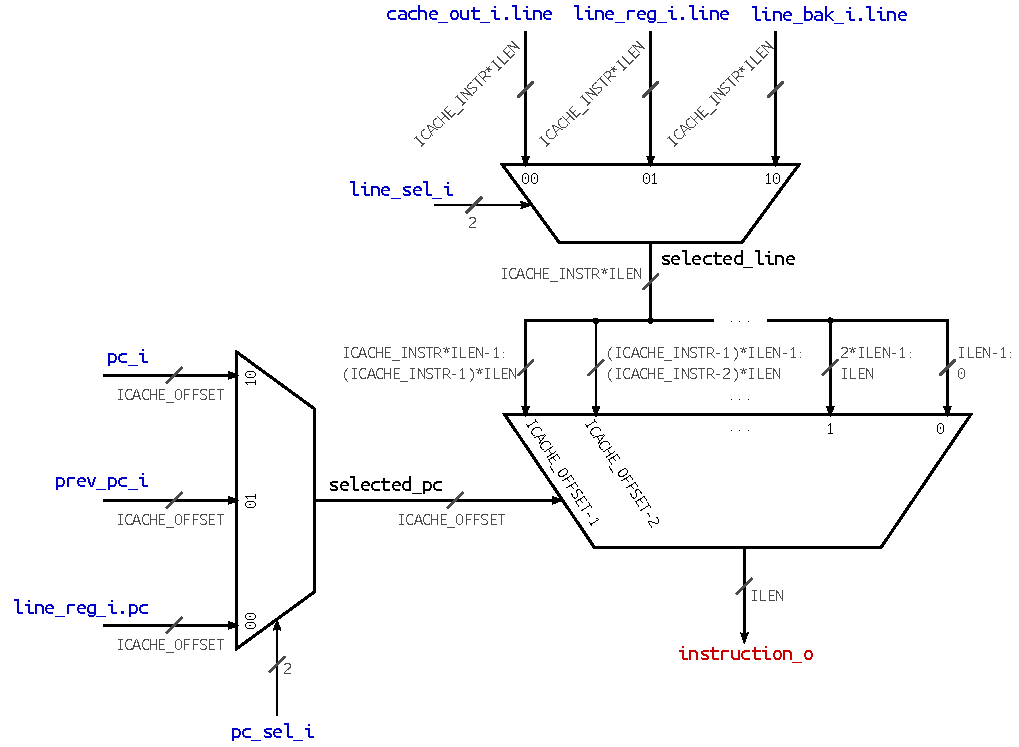
\includegraphics[width=\textwidth]{img/instr_sel.pdf}
  \caption{Selection network}
  \label{fig:instr_sel}
\end{figure}
The instruction selector takes as input all the three sources an instruction can be fetched from, three program counter sources\footnote{The only source actually used, as stated above, is the previous \ac{PC}, but the others were included in the initial version of the design and are kept should a future need arise. Given that the synthesizer can optimize unused wires, this choice incurs in no overhead.} and the respective selection signals (see \cref{fig:instr_sel-top}). It outputs a single selected instruction to be pushed to the issue queue.

\Cref{fig:instr_sel} shows the combinational selection network of the instruction selector, which basically consists of two multiplexers selecting the desired cache line and the address pointing to that line and another multiplexer choosing the selected instruction inside such line.

According to the number of instructions stored in a single cache line, the output multiplexed can become quite large, nonetheless it should not be an issue in terms of total area.

\subsection{Fetch controller}
\begin{figure}[hbt]
  \centering
  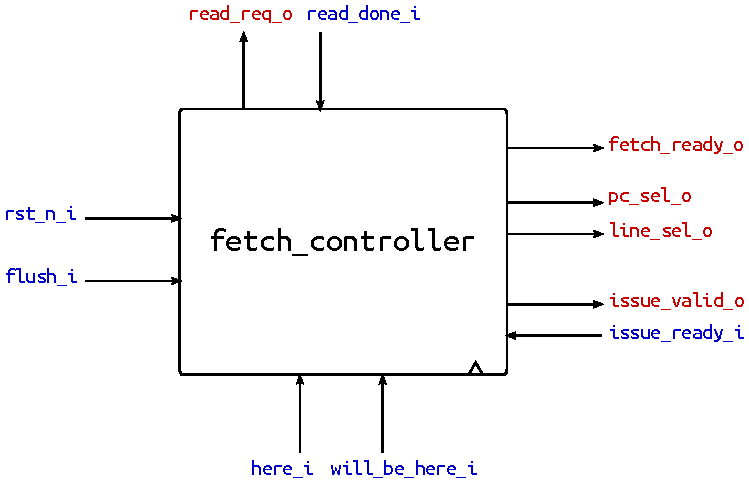
\includegraphics{img/fetch_controller-top.pdf}
  \caption{Fetch controller module ports}
  \label{fig:fetch_controller-top}
\end{figure}
The fetch controller module, whose interface is shown in \cref{fig:fetch_controller-top}, is the control unit of the \ac{IFU} which is responsible of receiving and generating control signals both for internal blocks and for interfacing with the other stages and the instruction cache. In particular, the controller receives information about saved instructions by the presence checker block (\texttt{here} and \texttt{will\_be\_here} signals) and as a consequence determines if a cache access is needed (\texttt{read\_req} and \texttt{read\_done} interface signals) and drives the correct selection signals (\texttt{pc\_sel} and \texttt{line\_sel}) to the instruction selector block.

Moreover, it handles the handshake signals \texttt{issue\_valid} and \texttt{issue\_ready} to and from the issue queue. The valid is asserted every time that the fetched instruction is available, as the result of a cache hit or saved in the line registers, while the ready signals that the issue queue is not full and has available room for one instruction. 

Finally, the \texttt{fetch\_ready} signal is used in the \ac{PC} gen stage as the enable of the output register (see \cref{fig:pc_gen_stage}) and in the fetch stage as the enable of the previous \ac{PC} register (see \cref{fig:ifu}). This signal is deasserted in the case of a stall, that in particular can occur if the cache misses on the requested address or if the issue queue is full and cannot accept more instructions. Note that in case of flush, however, this signal remains active, because the flush operation resets all the data structures in one clock cycle and at the next the \ac{IFU} is again ready to fetch, so the \ac{PC} gen stage must provide the new valid start address.

\subsubsection{Control unit}
The main difficulties reside in high number of possible combinations of events that can occur simultaneously. For instance the issue queue could become full while a memory access is being completed, or on the other hand while an instruction is being selected in the line register. These different conditions must be handled in a per-case manner and that is what the Mealy machine of \cref{fig:fetch_controller_fsm} manages. \todo{Why not Moore? Explain.} Follows a summary of the purpose of each state:
\begin{figure}[hbt]
  \centering
  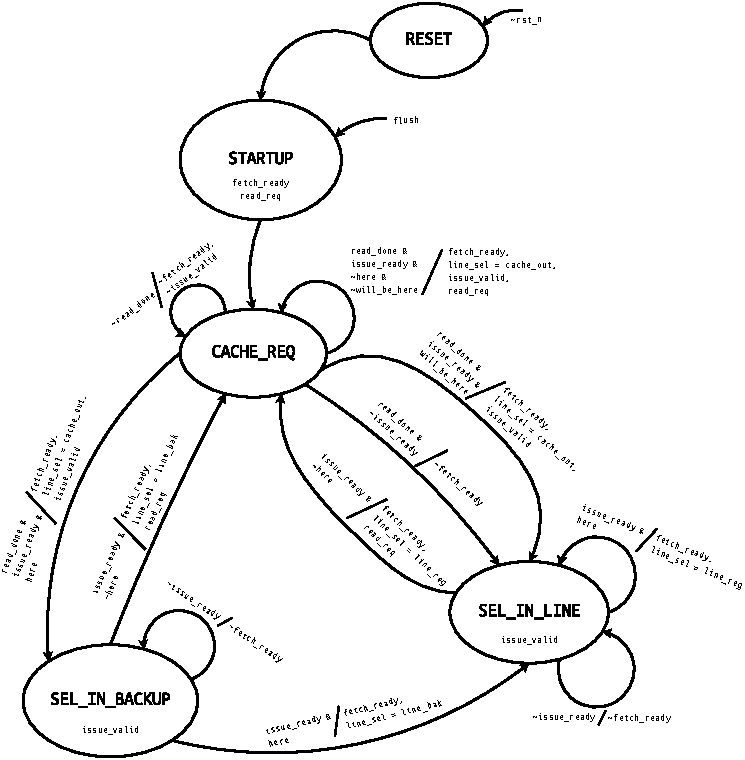
\includegraphics[width=\textwidth]{img/fetch_controller_fsm.pdf}
  \caption{Fetch controller \acs{FSM}}
  \label{fig:fetch_controller_fsm}
\end{figure}
\begin{itemize}
  \item \texttt{STARTUP}: this state can occur only after a reset or a flush. In both cases, at that moment the \ac{PC} corresponds to the starting address and all the line registers have been reset to zero, so a new cache read is necessary and the \texttt{read\_req} signal is asserted as a Moore output. The reason why the \ac{PC} is already valid and correct at this cycle is due to the fact that, in case of reset, the output register of the \ac{PC} gen stage is not reset to zero, but to the a constant \texttt{BOOT\_ADDRESS} that initiates the program execution. In case of flush, on the other hand, the \ac{PC} is set to the next address in the following cycle with respect to when the flush signal arrives, thanks to the OR gate (see \cref{fig:ifu}) that enables the \ac{PC} register in case of flush, even if the \texttt{fetch\_ready} signal would have prevented it. The latter is the other Moore output in this state and is needed, as stated before, to ensure maximum throughput before knowing if the cache will have a hit or miss (i.e. the next \ac{PC} is generated nonetheless and in case of miss the \ac{IFU} is stalled at the following cycle).
  \item \texttt{CACHE\_REQ}: in this state a memory access request is sent to the instruction cache interface. In case the cache is not ready to receive the address or incurs in a miss, then the \acs{FSM} loops in this state until the \texttt{read\_done} signals is asserted, stalling the frontend by deasserting \texttt{fetch\_ready}. 
  
  When the miss is resolved or immediately in case of hit, the state machine checks if the issue queue is ready. If it is, then the instruction is pushed and according to the output of the presence checker in that cycle, the next state transition is determined. If \texttt{here} is asserted, it means that the next instruction is present in the previously saved cache line, so at the next cycle, when the cache line just read will be saved in the line register and the old line register will be saved into the line backup register, the instruction will be selected from the backup register (move to \texttt{SEL\_IN\_BACKUP} state). If \texttt{will\_be\_here} is asserted, it means that the next instruction belongs to the same line that was just read, so it will be selected from the line register at the next cycle (move to \texttt{SEL\_IN\_LINE} state). If otherwise none of these signals are active, the next instruction belongs to a totally different cache line and so another memory access is necessary and the \acs{FSM} stays in this state.

  If the issue queue is full or busy, on the other hand, the cache output will be saved to the line register at the next cycle nonetheless, but the handshake with the queue does not take place and the state machine transitions to \texttt{SEL\_IN\_LINE} where it will loop until the issue queue becomes ready again. During this time, the line register will not be updated anymore as the fetch is stalled and no new memory accesses can be performed. \todo{Solution to mask a potential cache miss here?}
  \item \texttt{SEL\_IN\_LINE}: as mentioned above, in case the issue queue is busy, the \acs{FSM} loops in this state waiting. On the contrary, if the queue is ready, an instruction is pushed and then the state machine remains in this state if \texttt{here} is active, signaling that the next instruction will be selected from the same saved line, or moves to \texttt{CACHE\_REQ} otherwise to initiate a new cache request.
  \item \texttt{SEL\_IN\_BACKUP}: this state is the dual of \texttt{SEL\_IN\_LINE} meaning that the \acs{FSM} loops here when the issue queue is full and goes to \texttt{CACHE\_REQ} if the next instruction is not saved anywhere, but with the difference that, if the \texttt{here} signal is asserted, the next state is \texttt{SEL\_IN\_LINE}, where the instruction will be selected in the line register.
\end{itemize}

\subsubsection{Timing diagrams}
To better understand the behavior of the fetch controller \acs{FSM}, a list of timing diagrams covering a number of possible scenarios is now presented.

\begin{figure}[hbt]
  \centering
  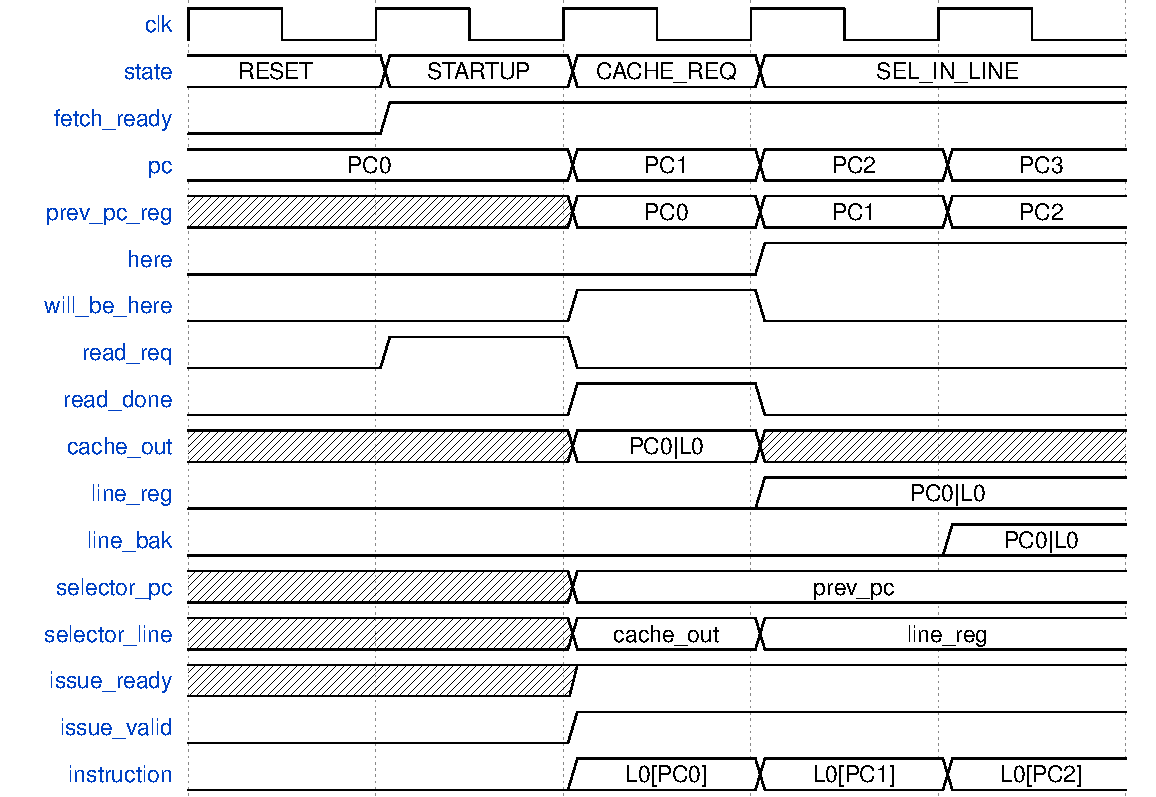
\includegraphics[scale=.6]{img/fetch01.pdf}
  \caption[Startup and hit]{Startup and hit (\texttt{PC0} is the \texttt{BOOT\_PC} considered above)}
  \label{fig:fetch01}
\end{figure}
\Cref{fig:fetch01} shows the boot up after the reset, where the first \ac{PC} needs a cache access and then the next instructions are fetched consecutively from the same line, now saved in the line register. This is the most ideal situation, with a cache hit and the issue queue ready. It is clear from this timing diagram that the \texttt{fetch\_ready} signal must be active during \texttt{STARTUP} even if the outcome of the cache request is not yet known. If this were not the case, there would be a one-cycle penalty every time.

\begin{figure}[!h]
  \centering
  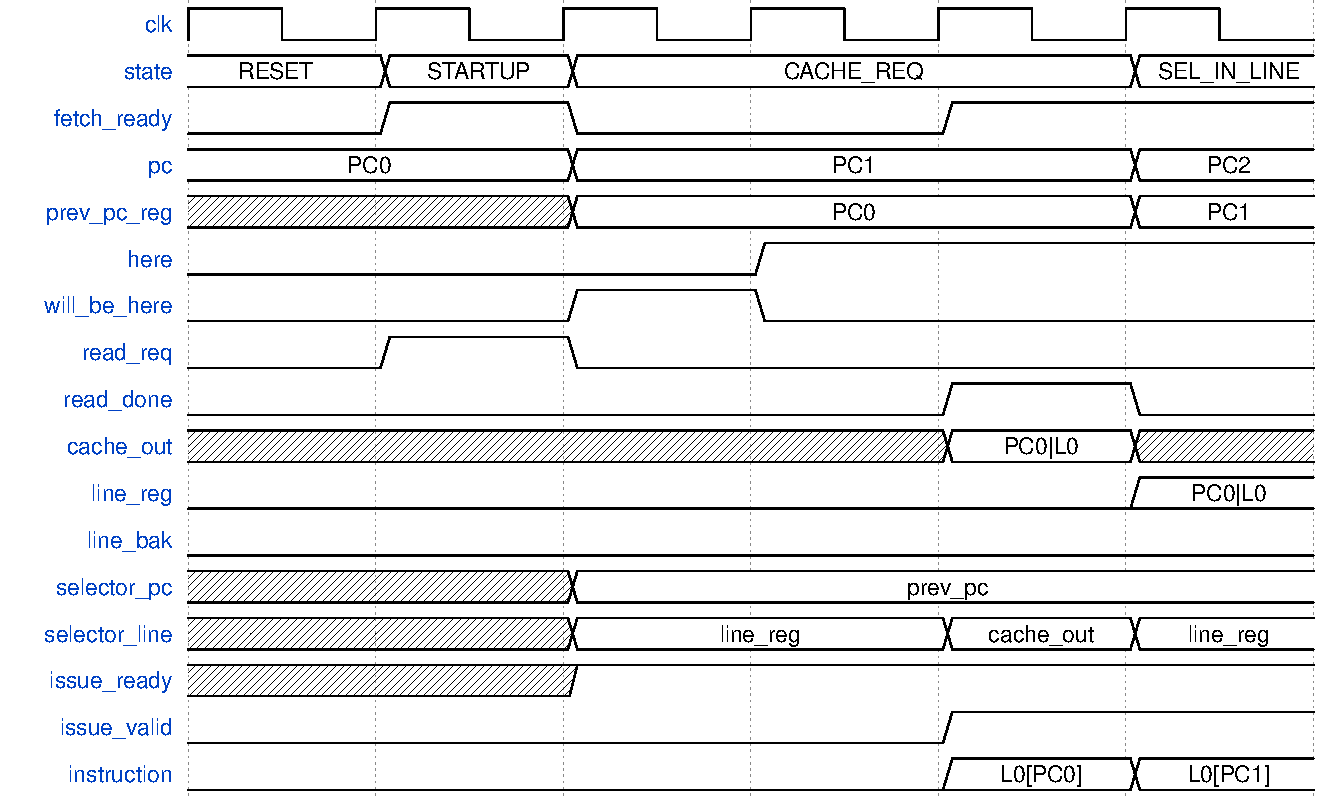
\includegraphics[scale=.6]{img/fetch02.pdf}
  \caption{Startup and cache not ready/miss}
  \label{fig:fetch02}
\end{figure}
\Cref{fig:fetch02} shows what happens in the same situation if instead the cache is not ready or has a miss. This timing also explains why the instruction cache interface must save the address as soon as a read request is sent: if the address handshake does not occur at the second cycle when the request is made, then the address changes at the next clock and the read would happen at the new, wrong address.

\begin{figure}[!h]
  \centering
  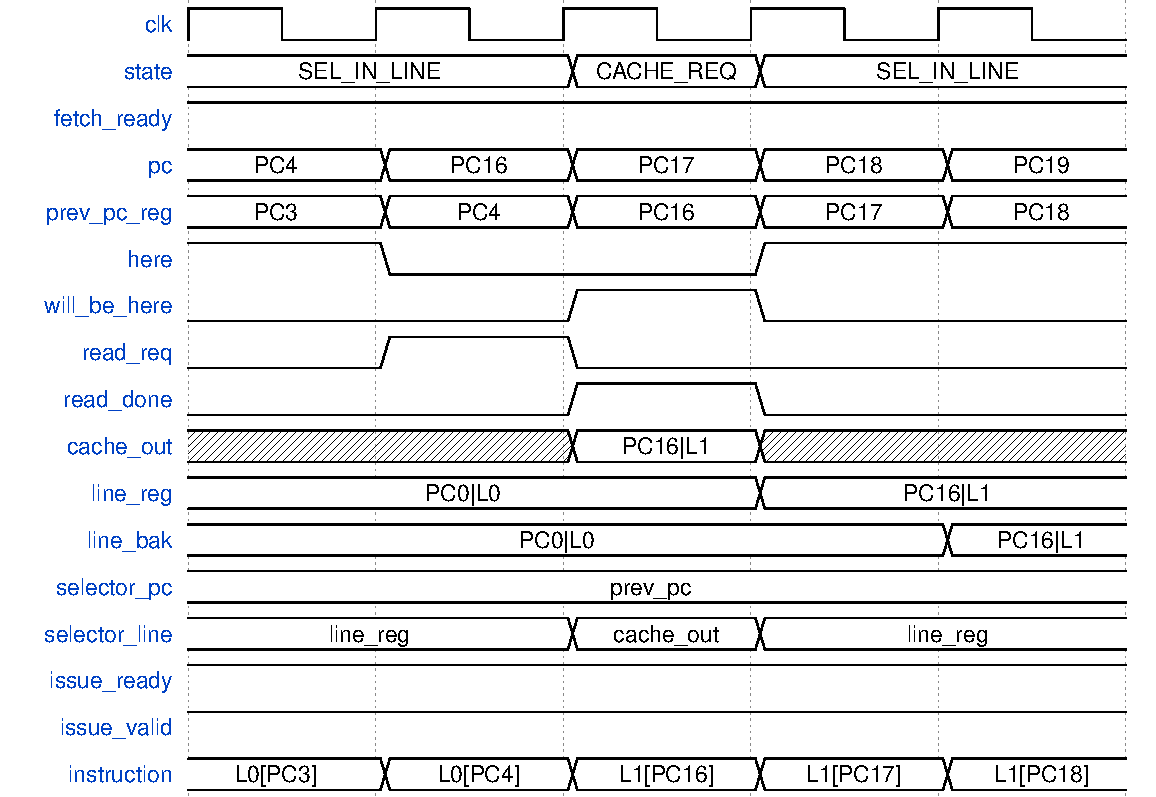
\includegraphics[scale=.6]{img/fetch06.pdf}
  \caption{Saved line change}
  \label{fig:fetch06}
\end{figure}
\Cref{fig:fetch06} shows the situation of a cache line change. At first instructions are read consecutively from the line register, then a branch for example makes the \ac{PC} jump to a location stored on a different cache line, so a read request is sent, the cache hits and the current instruction is read from the cache output. After that, fetch continues sequentially with the other instructions in the new saved line.

\begin{figure}[!h]
  \centering
  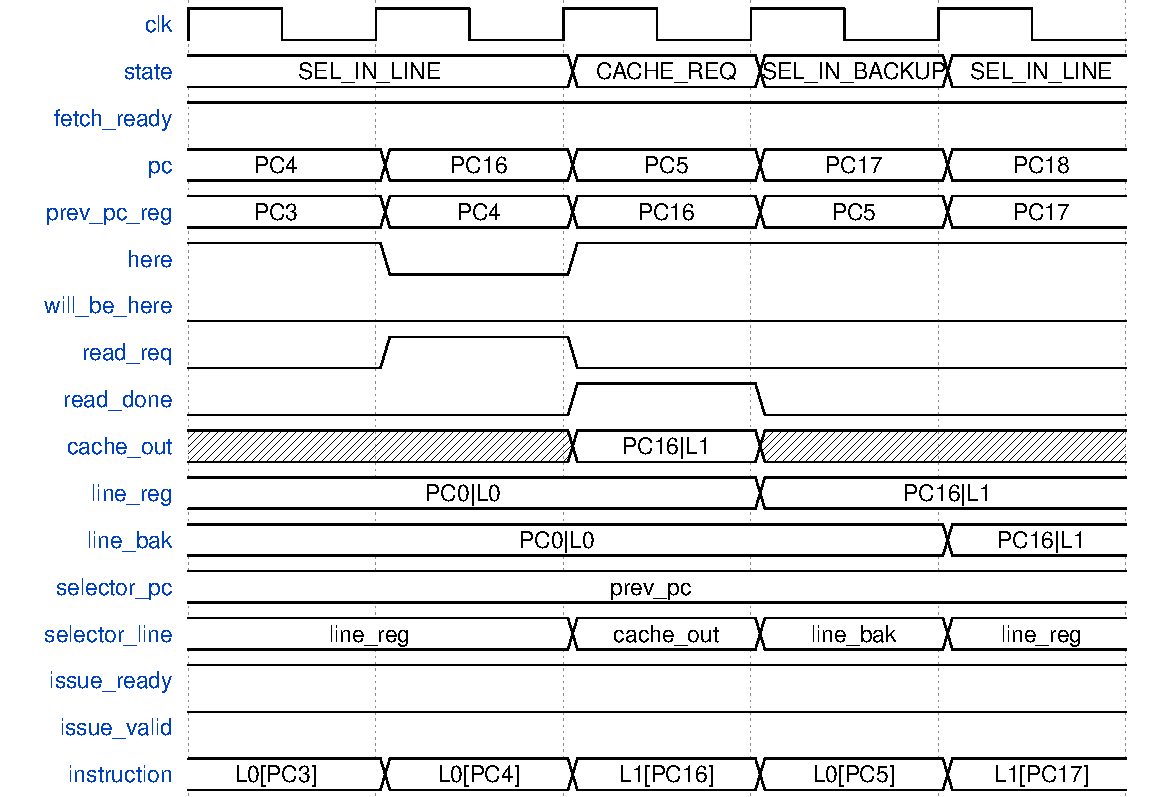
\includegraphics[scale=.6]{img/fetch09.pdf}
  \caption{Line backup register purpose}
  \label{fig:fetch09}
\end{figure}
The purpose of the line backup register is demonstrated in the timing of \cref{fig:fetch09}, when there is a jump back and forth between two cache lines: the \texttt{here} signal during the cache request makes the next instruction be selected from the backup register. Of course, as already mentioned, the limitation of this solution is that if the same jump were to happen just right after this scenario (e.g. if \texttt{PC5} arrived again instead of \texttt{PC18} at the last shown cycle) even the backup register would have been overwritten and so a new memory access would be needed anyway.

\begin{figure}[!h]
  \centering
  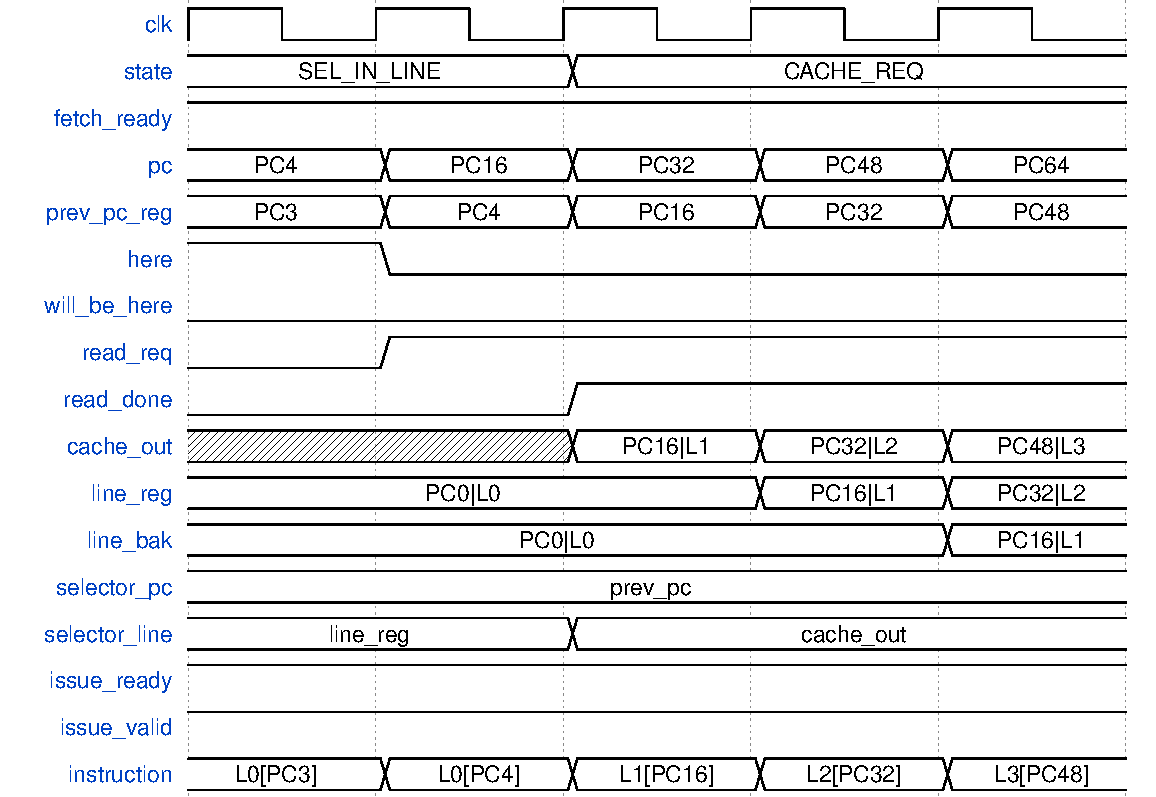
\includegraphics[scale=.6]{img/fetch07.pdf}
  \caption{Cache read pipeline}
  \label{fig:fetch07}
\end{figure}
\Cref{fig:fetch07} illustrates the ability to reach a throughput on one instruction per clock cycle in a pipeline even while reading from the instruction cache, if the memory hits on every address. In this case instructions are always selected directly from the cache output.

\begin{figure}[!h]
  \centering
  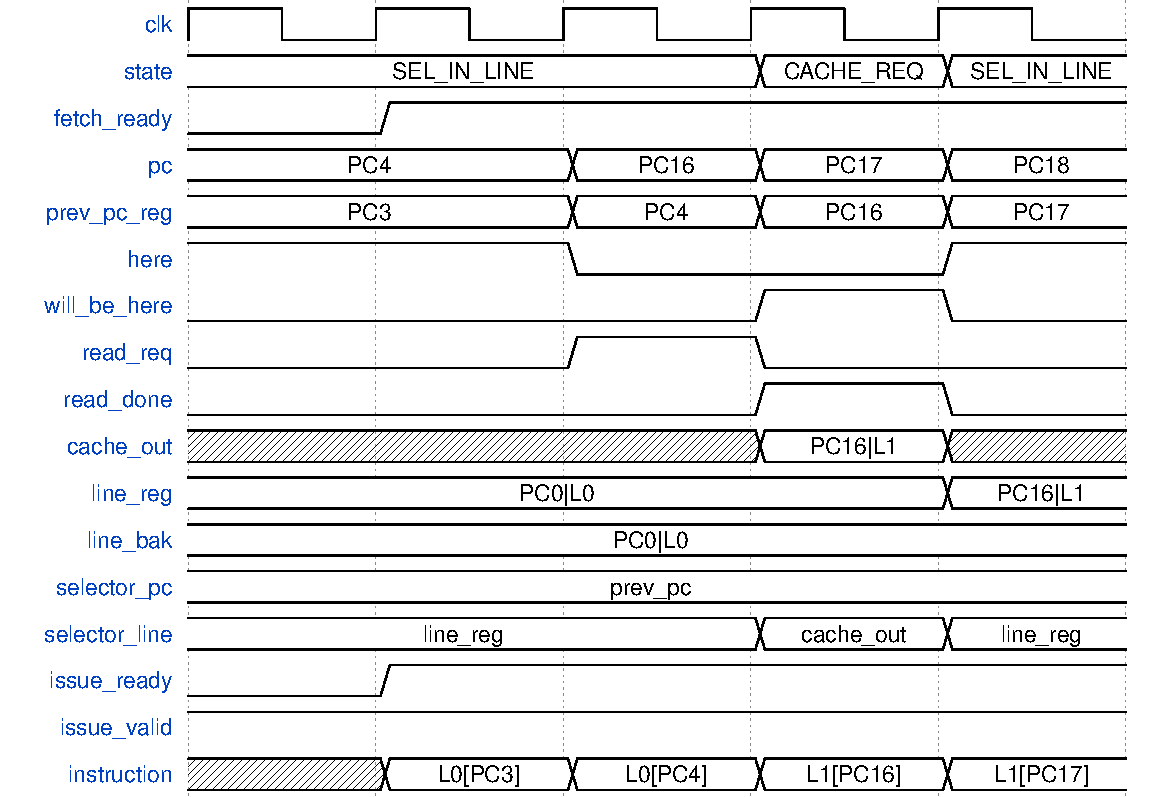
\includegraphics[scale=.6]{img/fetch03.pdf}
  \caption{Issue queue not ready during selection}
  \label{fig:fetch03}
\end{figure}
\begin{figure}[!h]
  \centering
  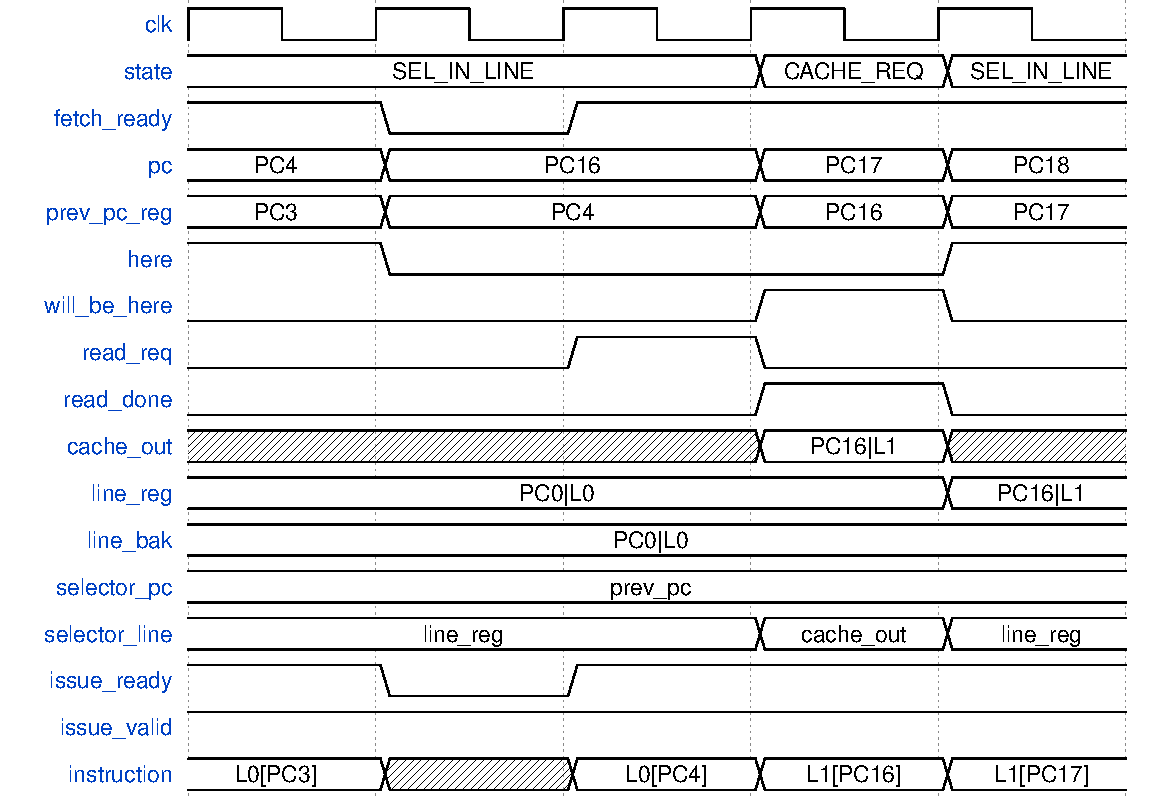
\includegraphics[scale=.6]{img/fetch04.pdf}
  \caption{Issue queue not ready during request}
  \label{fig:fetch04}
\end{figure}
\Cref{fig:fetch03,fig:fetch04} show the issue queue being not ready at two different instants. In \cref{fig:fetch03} the stall happens when the instruction is selected inside the line register and in this case no problem arises, as the fetch stage is simply stalled and no register changes until the issue queue becomes ready again. If the queue is busy when an address would require a cache read, as in \cref{fig:fetch04}, then the actual memory access is delayed until this stall is resolved. \todo{C'mon, solve this} In both cases, the \texttt{fetch\_ready} signal is deasserted to prevent the generation of new program counters.

\begin{figure}[!h]
  \centering
  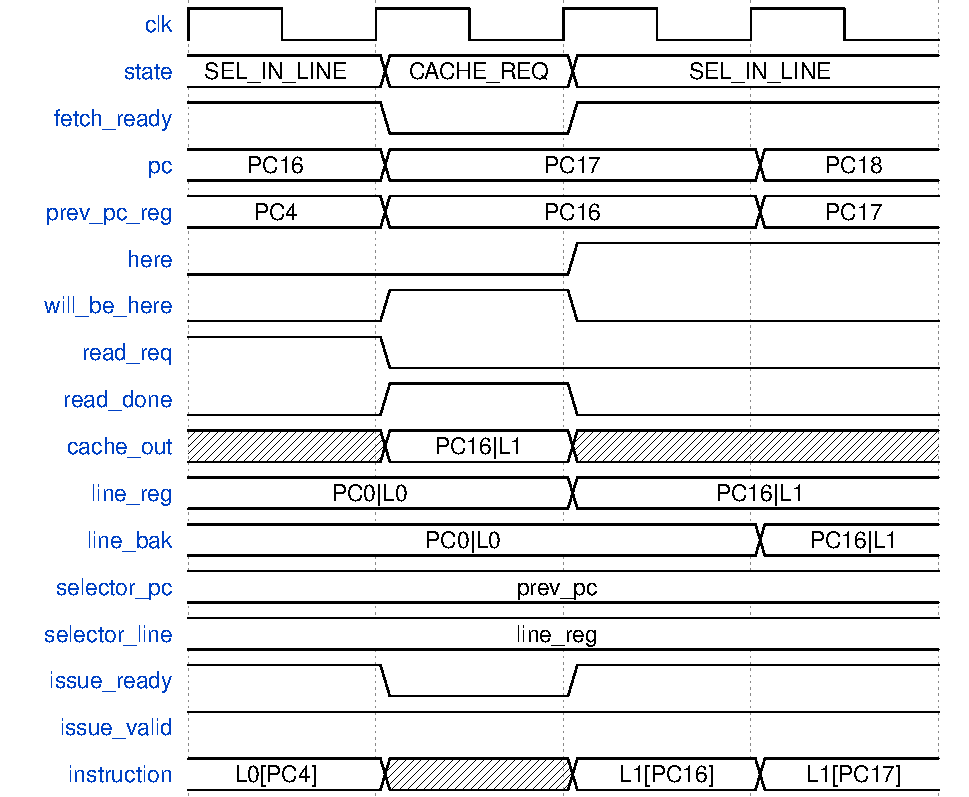
\includegraphics[scale=.6]{img/fetch05.pdf}
  \caption{Issue queue not ready when cache line arrives}
  \label{fig:fetch05}
\end{figure}
\Cref{fig:fetch05} shows the case for which the issue queue is not ready when the cache hits and outputs a new line and the current address points to an instruction in that line (\texttt{will\_be\_here} asserted). In this case, there is a stall when no new \ac{PC} is generated and during which the newly read line is saved into the line register, so that when the issue queue becomes ready again the instruction will be selected from the register and not from the cache output.

\begin{figure}[!h]
  \centering
  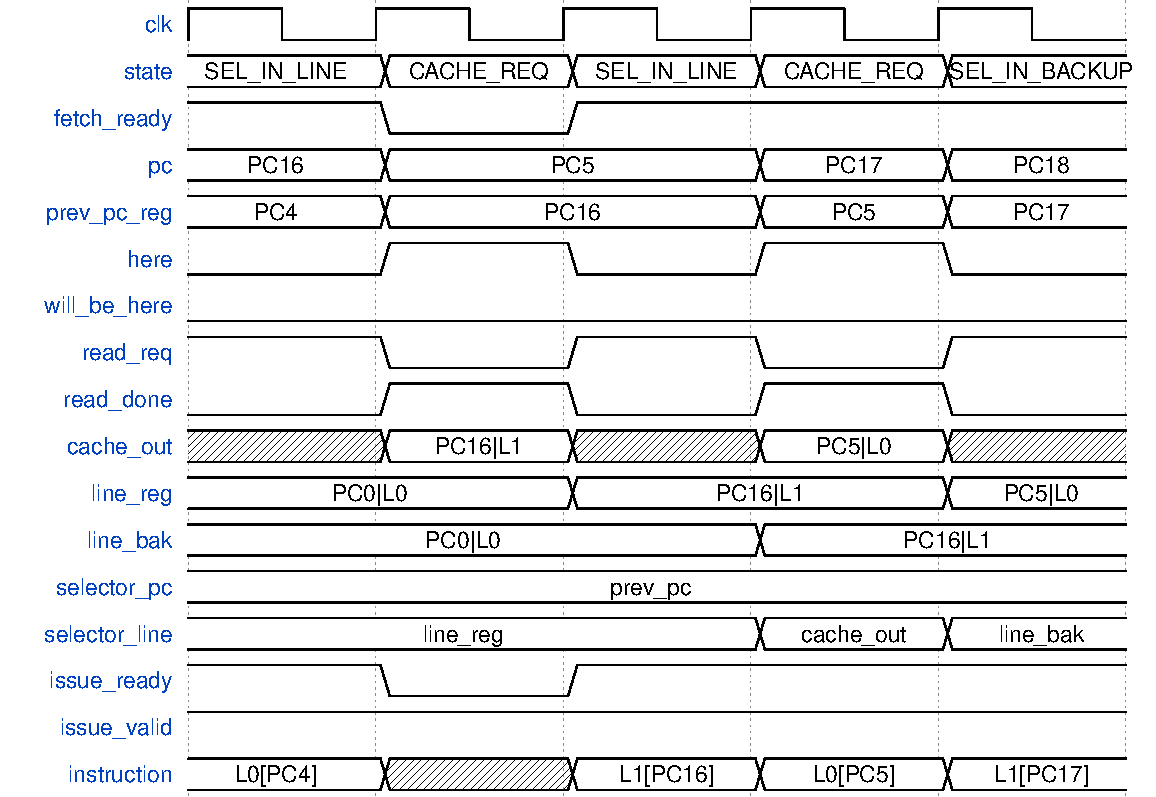
\includegraphics[scale=.6]{img/fetch08.pdf}
  \caption{Issue queue not ready and causing of backup}
  \label{fig:fetch08}
\end{figure}
The situation shown in \cref{fig:fetch08} is similar to the previous one, but this time the issue queue is not ready when the outputs a new line and the current instruction refers to a line previously saved. In this case not even the line backup register can manage it, as as soon as the fetch resume, it is updated with the content of the line register, that is the last cache line read. So, for the old line a new memory access is required.

\begin{figure}[!h]
  \centering
  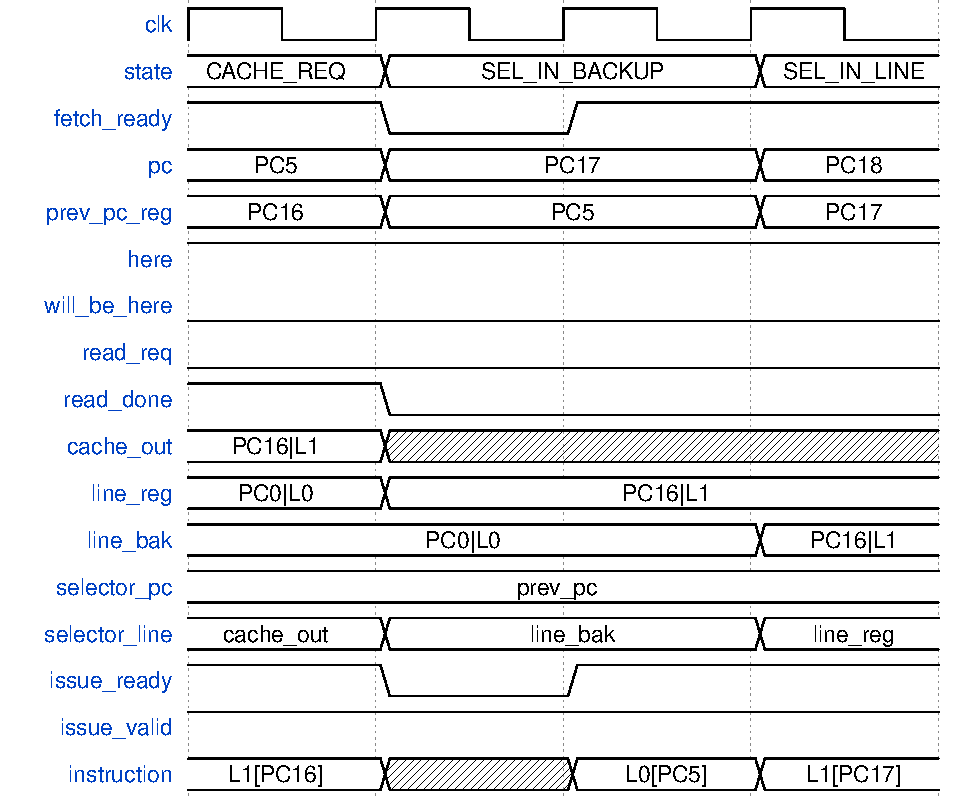
\includegraphics[scale=.]{img/fetch10.pdf}
  \caption{Issue queue not ready during backup}
  \label{fig:fetch10}
\end{figure}
Finally, \cref{fig:fetch10} shows the last timing under analysis, that is the situation in which the issue is not ready when the instruction has to be selected inside the backup register. In similar manner to \cref{fig:fetch03}, here the stall does not cause any issues and the fetch resumes exactly as before when the queue turns ready again.

\pagebreak
\section{\acf{BPU}}
As seen in \cref{fig:frontend}, the \ac{BPU} resides in the fetch stage and works in parallel with the \ac{IFU} on each address coming from the \ac{PC} gen stage. This unit, as shown in the high level scheme of \cref{fig:bpu-idea}, is composed of two main blocks:
\begin{figure}[hbt]
  \centering
  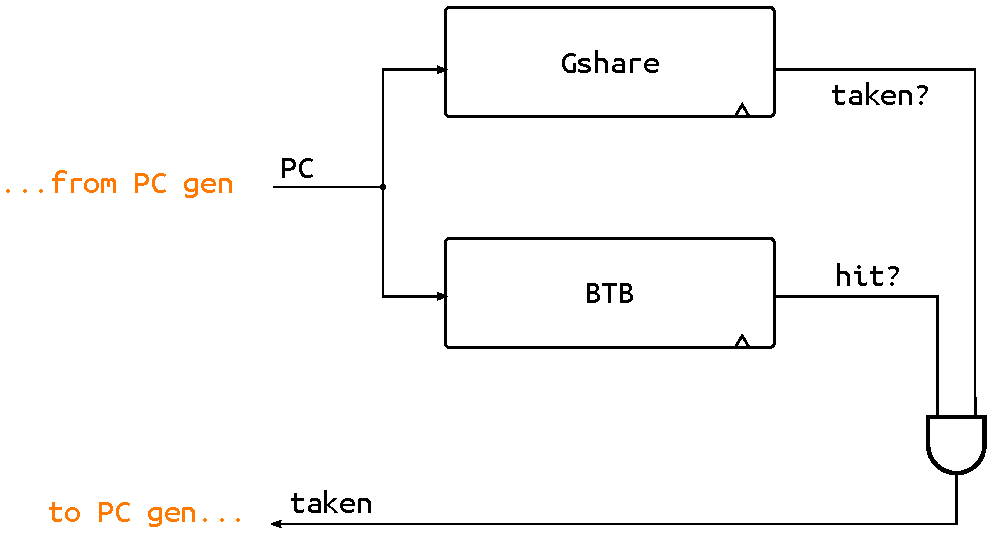
\includegraphics[width=.8\textwidth]{img/bpu-idea.pdf}
  \caption{\acs{BPU} general idea}
  \label{fig:bpu-idea}
\end{figure}
\begin{itemize}
  \item The \textbf{gshare} is the actual branch predictor and is a variation of the two-level predictor described in \cref{sec:twolevelbp} featuring a table of 2-bit counters and a global history register, of which a detailed explanation is provided in \cref{sec:gshare}. Being a branch predictor, its output is the predicted direction of the branch. Note that it outputs a prediction on every address, even those who potentially do not correspond to branch instructions. That is where the second block comes into play.
  \item The \textbf{\acf{BTB}}, described in \cref{sec:btb}, is a small cache that contains the target address of taken branches only. This provides the significant advantage of being able to fetch the instruction after the taken branch with no additional delay, leading to zero overhead branches if the target is correct.
\end{itemize}
A branch is predicted taken by the \ac{BPU} if and only if the gshare predictor supposes the branch is taken and the \ac{BTB} contains an entry with a valid address for that specific \ac{PC}.

\subsection{Top-level block diagram}
\begin{figure}[hbt]
  \centering
  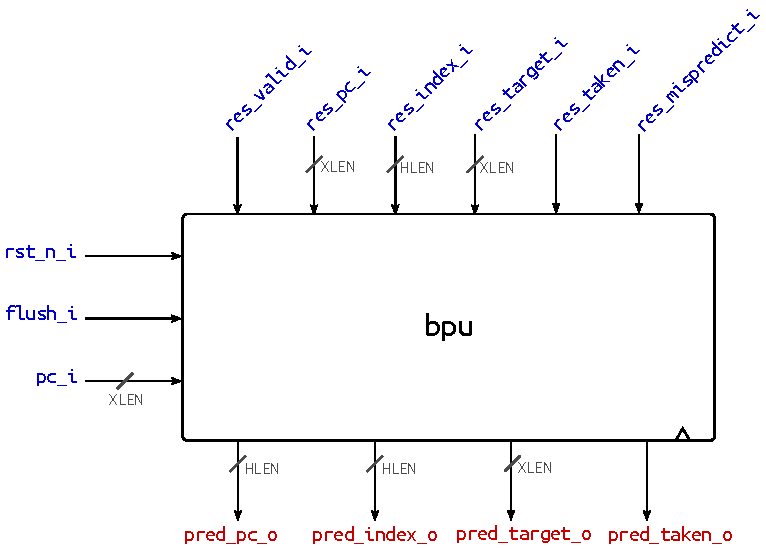
\includegraphics[width=.9\textwidth]{img/bpu-top.pdf}
  \caption{\acs{BPU} module ports}
  \label{fig:bpu-top}
\end{figure}
\Cref{fig:bpu-top} shows the module interface of the \ac{BPU}. Apart from reset and flush signals, used respectively at startup and in case an exception requires the internal data structures to be flushed, the module outputs a prediction based on the current address, composed by a single bit indicating if the branch is supposed to be taken or not, the predicted target and also the branch address, which is later needed to update the predictor structures.

The inputs containing the \texttt{res} prefix, for resolution, are the just mentioned branch \ac{PC} to which the resolution refers, the actual target, the actual branch direction, a bit indicating if there was a misprediction and a valid bit to signal that the present one is a valid branch resolution coming from the execution stage.

\begin{table}[hbt]
  \centering
  \makebox[\textwidth][c]{
    \begin{tabular}{llll}
      \toprule
      \textbf{Prediction}         & \textbf{Resolution}         & \textbf{Target}             & \textbf{Action} \\
      \midrule
      Taken                       & Taken                       & Correct                     & Increment 2-bit counter \\
      \midrule
      \multirow{3}{*}{Taken}      & \multirow{3}{*}{Taken}      & \multirow{3}{*}{Incorrect}  & Increment 2-bit counter \\
                                  &                             &                             & Update BTB entry \\
                                  &                             &                             & Flush pipeline and restart from correct target \\
      \midrule
      \multirow{3}{*}{Taken}      & \multirow{3}{*}{Not taken}  & \multirow{3}{*}{--}         & Decrement 2-bit counter \\
                                  &                             &                             & Remove BTB entry \\
                                  &                             &                             & Flush pipeline and restart from branch \ac{PC}+4 \\
      \midrule
      Not taken                   & Not taken                   & --                          & Decrement 2-bit counter \\
      \midrule
      \multirow{3}{*}{Not taken}  & \multirow{3}{*}{Taken}      & \multirow{3}{*}{--}         & Increment 2-bit counter \\
                                  &                             &                             & Add BTB entry \\
                                  &                             &                             & Flush pipeline and restart from correct target \\
      \bottomrule          
    \end{tabular}
  }
  \caption{Predictor update actions}
  \label{tab:bpupdate}
\end{table}
This information, in particular the two bits about the actual branch direction and the misprediction, is used to update the data structures and take further action as listed in \cref{tab:bpupdate}. In case of correct prediction, it is only needed to update the 2-bit counters inside the gshare predictor according to the branch direction. A misprediction, on the other hand, requires different actions to be taken depending on which event caused it. If the branch was correctly predicted taken, but the target in the \ac{BTB} was incorrect, then the \ac{BTB} entry must be updated with the correct one. If, instead, the branch was mispredicted taken, the target buffer entry is deleted in order to prevent a potential further misprediction, in the case when the 2-bit counter was in the \emph{strongly taken} state. Finally, if the branch was mispredicted not taken, then the corresponding target is added to the \ac{BTB}. This time, if the 2-bit counter was in the \emph{strongly not taken} state, the second misprediction cannot be prevented and the same entry will be written once again in the \ac{BTB}.

In all the misprediction cases, the fetch and execution stages must be flushed and the next \ac{PC} must be set to the next sequential address after the branch \ac{PC} if the branch was actually not taken, or to the correct target if the branch was actually taken. Note that this flush operation is different from the flush caused by an exception because, obviously, it does not reset the branch predictor structures, which are only updated with the correct branch result.

\begin{figure}[!h]
  \centering
  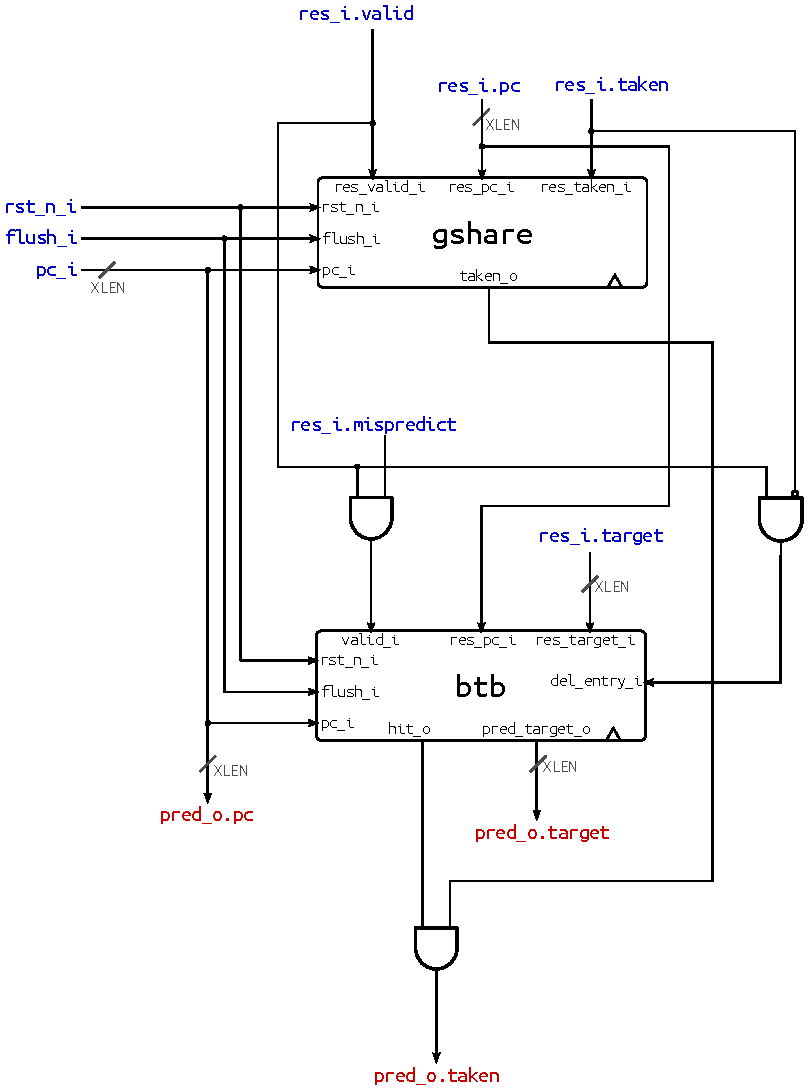
\includegraphics[width=\textwidth]{img/bpu.pdf}
  \caption{\acs{BPU} block diagram}
  \label{fig:bpu}
\end{figure}
\Cref{fig:bpu} shows the internal organization of the \ac{BPU} which is simply composed of the gshare and \ac{BTB} blocks, along with the AND gate of \cref{fig:bpu-idea} and a couple of other gates to decide the correct update action based on the results, as in \cref{tab:bpupdate}.

\subsection{Gshare branch predictor}\label{sec:gshare}
\begin{figure}[hbt]
  \centering
  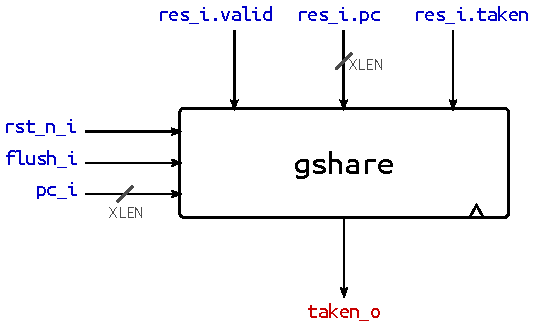
\includegraphics{img/gshare-top.pdf}
  \caption{Gshare module ports}
  \label{fig:gshare-top}
\end{figure}
The idea of the gshare predictor, whose interface is shown in \cref{fig:gshare-top}, was first proposed by Scott McFarling in a 1993 paper \cite{mcfarling93} and consists in a variation of the two-level predictor that combines global information from the global branch history and local information of the current branch address by hashing them with the exclusive OR of the history register and the $N$ least significant bits of the \ac{PC}, where $N$ is the history length. \todo{Expand a little on gshare?}

\begin{figure}[hbt]
  \centering
  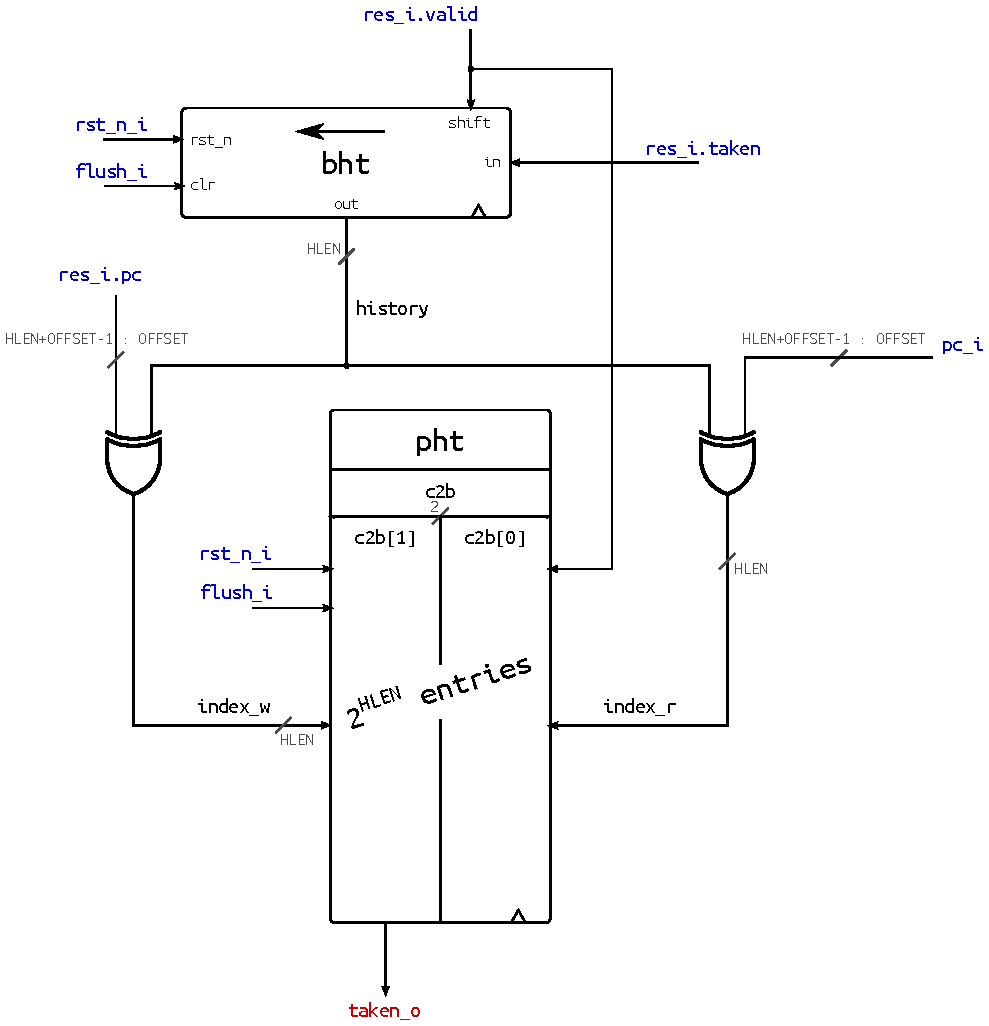
\includegraphics[width=.9\textwidth]{img/gshare.pdf}
  \caption{Gshare branch predictor}
  \label{fig:gshare}
\end{figure}
The structure of this predictor is shown in \cref{fig:gshare} and is composed of a \ac{BHT} composed of a single shift register where branch resolutions are left shifted in and a \ac{PHT} that contains an array of 2-bit counters, organized as a register file, so providing synchronous write and asynchronous read. This table is indexed by the XOR of the history and the current \ac{PC}\footnote{Actually, the 2 \acsp{LSB} of the \ac{PC} are excluded as are always zero for 32-bit instruction.} in order to read the prediction for the current branch, which comes from the most significant bit of the 2-bit counter.

\begin{figure}[hbt]
  \centering
  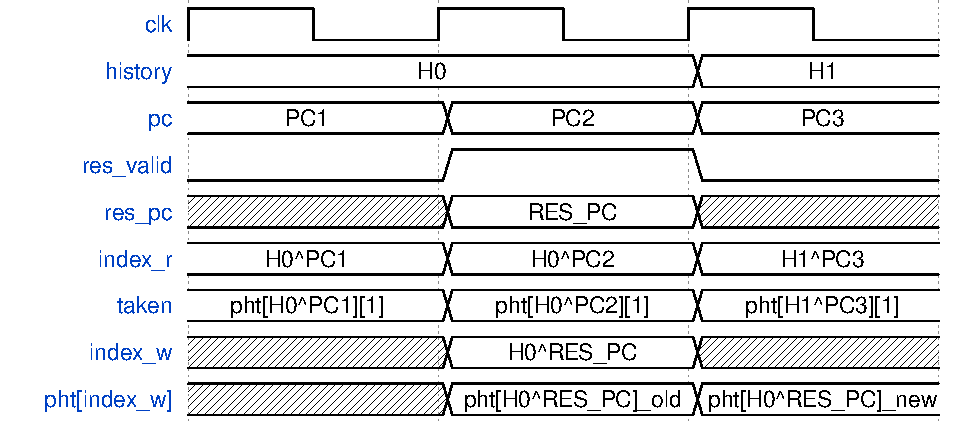
\includegraphics[width=.8\textwidth]{img/gshare01.pdf}
  \caption{Update timing diagram}
  \label{fig:gshare01}
\end{figure}
To update the \ac{PHT} when a branch is resolved the correct 2-bit counter has to be selected using the same index as the one used for the prediction. As an architectural choice, branches in LEN5 are resolved in-order during the execution stages, so that in the time span between the prediction and the resolution of a branch, no other resolution is generated and as such the branch history remains unchanged. This means that the write index used to select the 2-bit counter to be updated can be derived using the resolved branch address and the same current value of the history register. This poses no timing issues, as demonstrated by \cref{fig:gshare01}, because the history register is shifted only after the clock edge when the \texttt{res\_valid} signal is active, so at that edge the register still stores the unshifted value and the write operation on the \ac{PHT} occurs at the correct address.

If branches were resolved \ooo, on the other hand, to restore the correct address to the \ac{PHT} the index at the moment of the prediction would need to be passed along in the pipeline to return at the moment of the resolution. \todo{So why in-order branches?}

The initial version of the design also accounted for a column of valid bits in the \ac{PHT} to indicate if the prediction coming from each 2-bit counter is valid (i.e. if that 2-bit counter has already been used at least once). This is useful to prevent taken misprediction if the 2-bit counters are initialized in the weakly or strongly taken state. However, if the counters are instead initialized in a not taken state, then the first time they are accessed the prediction will always be ``not taken'' just as if the valid bit was included, so this bit becomes redundant and only wastes area. After a more thorough analysis, presented in \cref{sec:}, it was decided to remove the valid bits from the \ac{PHT}.

\subsection{\acf{BTB}}\label{sec:btb}
\begin{figure}[hbt]
  \centering
  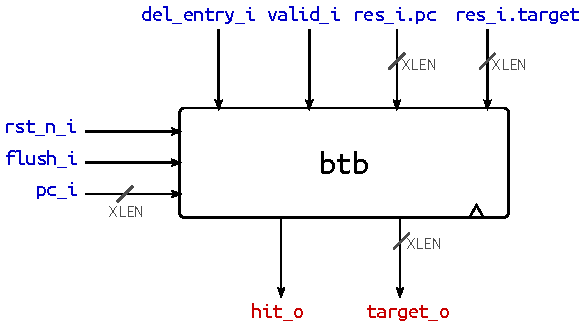
\includegraphics{img/btb-top.pdf}
  \caption{\acs{BTB} module ports}
  \label{fig:btb-top}
\end{figure}
\begin{figure}[hbt]
  \centering
  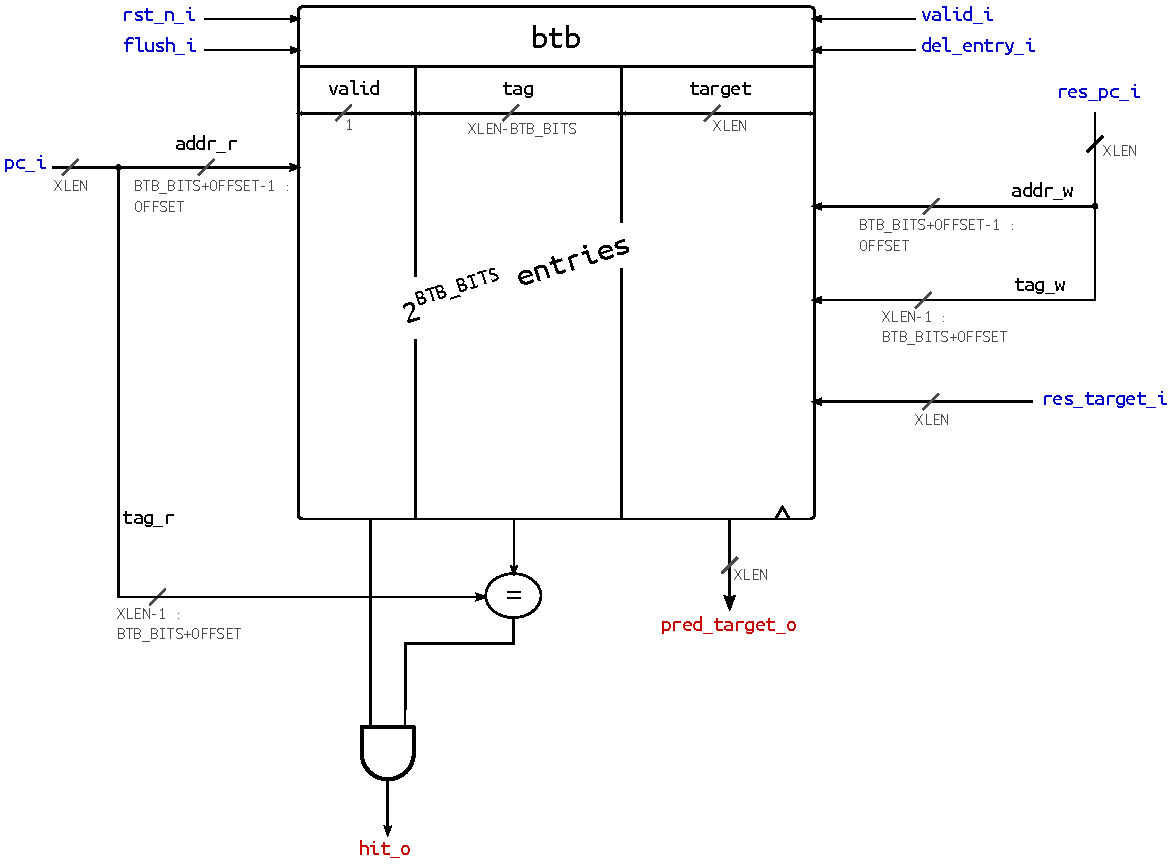
\includegraphics[width=\textwidth]{img/btb.pdf}
  \caption{\acs{BTB} diagram}
  \label{fig:btb}
\end{figure}
The purpose of the \ac{BTB} (interface in \cref{fig:btb-top}) is to provide the target of a predicted taken branch in order to eliminate the delay of the computation of the destination address in the later execution stages and allow the fetch to proceed immediately from the new address. The idea of a \ac{BTB} was first introduced in \cite{lee84} and was since optimized and employed a great number of processor designs.

Its structure shown in \cref{fig:btb} is basically that of a direct mapped cache with $2^{\texttt{BTB\_BITS}}$ entries addressed using the the \texttt{BTB\_BITS} least significant bits of the \ac{PC}, as always excluding the offset, where each of them contains the following fields:
\begin{itemize}
  \item \textbf{Valid}: 1-bit field indicating if the selected entry is valid, that is if it has been previously written with the correct target of a resolved branch.
  \item \textbf{Tag}: this field contains the remaining bits of the branch \ac{PC} not used to address the \ac{BTB}. The final evaluation on the branch address is a hit only if for the selected location the valid bit is set and the stored tag corresponds to the upper part of the \ac{PC}. This is done in order to eliminate the aliasing phenomenon, for which multiple addresses could point to the same \ac{BTB} entry and thus produce incorrect results for the target. 
  \item \textbf{Target}: the actual destination address of the branch. The 2 \acsp{LSB} are not stored as are they are useless for 32-bit instructions, but can save a significant amount of area if the \ac{BTB} contains many entries.
\end{itemize}
When the \texttt{del\_entry} signal is asserted all three fields of the addressed entry are reset to zero.

The \ac{BTB} is perhaps one of the blocks that can organized and optimized in the most number of ways, starting from the mapping of the cache to the information stored. Some variants of the design store the actual target instruction instead of the address to allow for some advanced techniques such as branch folding \cite{perleberg93}. Being LEN5 an exploratory experiment on processor design, the choice has been made to keep the organization simple and so implement the \ac{BTB} as a direct mapped cache described as a register file.

For this reason, the same principles presented in \cref{sec:gshare} apply here, namely that the \ac{BTB} allows synchronous write and asynchronous read that in turn imply that a prediction and an update can be completed during the same cycle.

\section{Branch unit}
A unit that was not talked about until now and that is not shown in \cref{fig:frontend} because it resides in the backend is the branch unit, which is an execution unit responsible of determining the actual outcome of branch instructions. Its main tasks are the logic comparison between operand values in order to determine if the branch is taken or not and the sum of the base branch address and its immediate field to discover the target.

\begin{figure}[hbt]
  \centering
  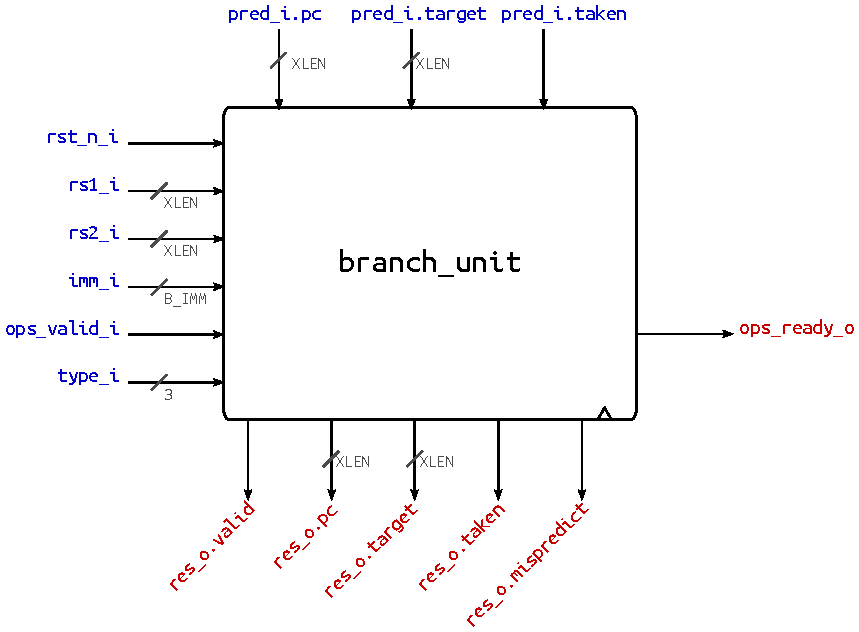
\includegraphics[width=.9\textwidth]{img/branch_unit-top.pdf}
  \caption{Branch unit module ports}
  \label{fig:branch_unit-top}
\end{figure}
\Cref{fig:branch_unit-top} shows the interface ports of this unit. It receives the register operands \texttt{rs1} and \texttt{rs2}, the immediate field \texttt{imm} the branch type, encoded on three bits, and the prediction information from the corresponding reservation station, to and from which it communicates via the handshake signals \texttt{ops\_valid} and \texttt{ops\_ready} as usual.

Its outputs are the information on the branch resolution, which is passed forward to the commit stage and back to the frontend to update the \ac{BPU} and potentially stall in case of misprediction.

\subsection{Datapath}
\begin{figure}[hbt]
  \centering
  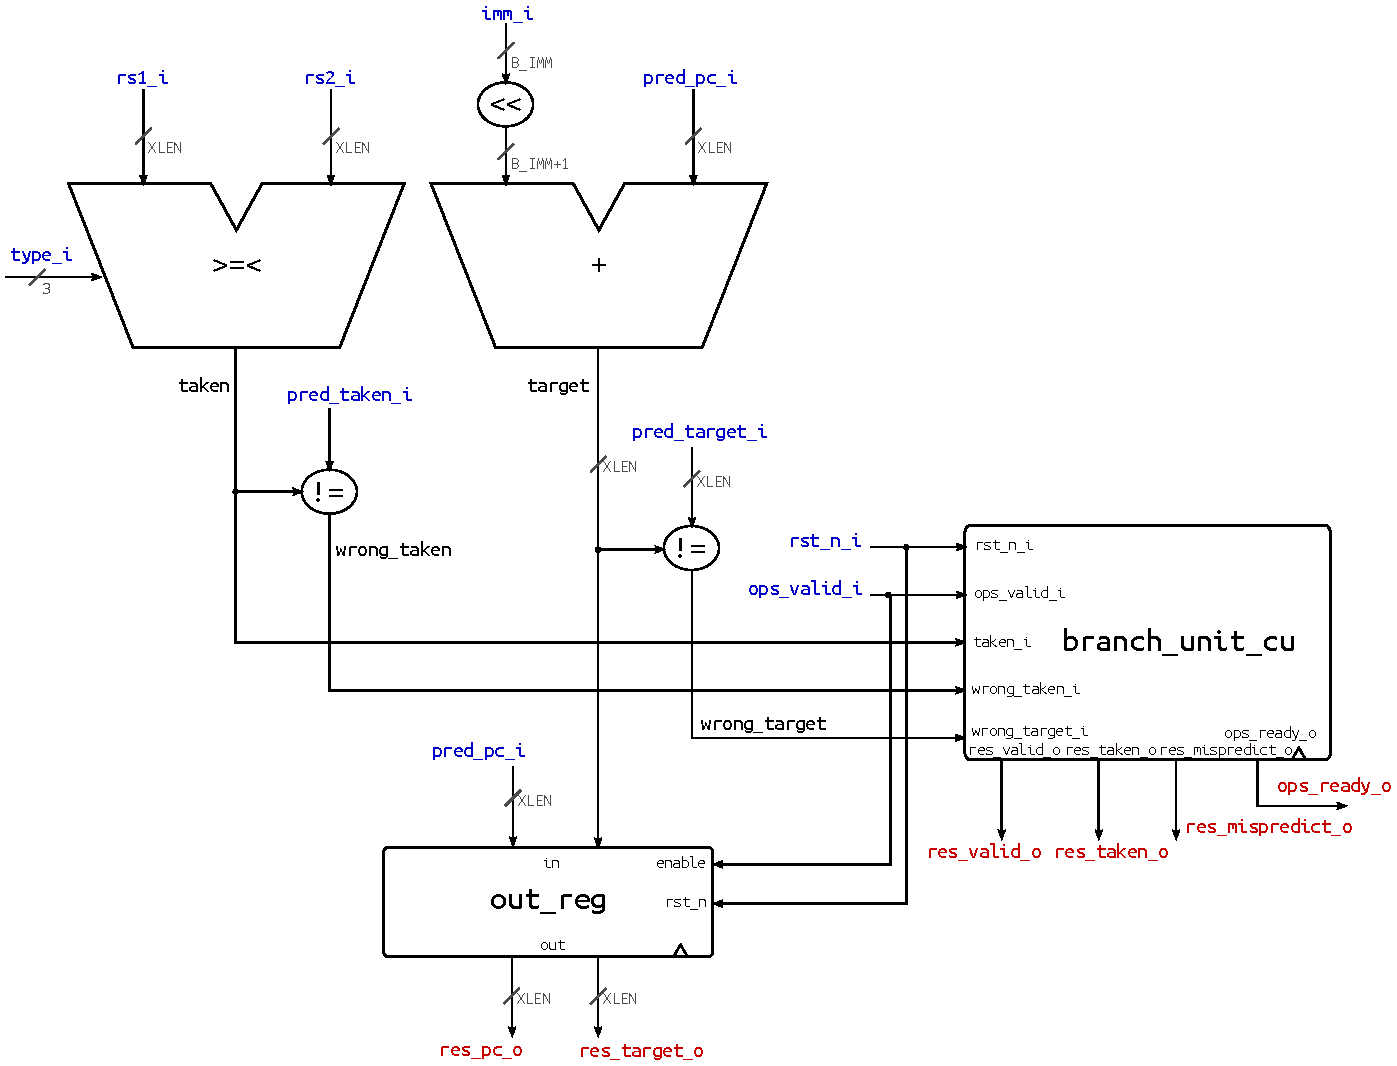
\includegraphics[width=\textwidth]{img/branch_unit.pdf}
  \caption{Branch unit datapath}
  \label{fig:branch_unit}
\end{figure}
The datapath of the branch unit is shown in \cref{fig:branch_unit} and is composed of two \acsp{ALU}, which are actually a separate logic unit and an adder, operating in parallel on the comparison and the target computation, which is performed, as per \riscv specifications, by adding the base address with the immediate left shifted. The output of both units is compared with the predicted taken and target respectively and the results are passed to the control unit.

There are six types of branches in the \riscv \ac{ISA}, namely:
\begin{itemize}
  \item Branch if equal (\texttt{BEQ})
  \item Branch if not equal (\texttt{BNE})
  \item Branch if less than (\texttt{BLT})
  \item Branch if greater than or equal (\texttt{BGE})
  \item Branch if less than, unsigned (\texttt{BLTU})
  \item Branch if greater than or equal (\texttt{BGEU})
\end{itemize}

At the following clock cycle after the \acsp{ALU} have obtained the results, the control unit outputs the correct prediction information and the branch \ac{PC} and right target are written to the output register.

\subsection{Control unit}
\begin{figure}[hbt]
  \centering
  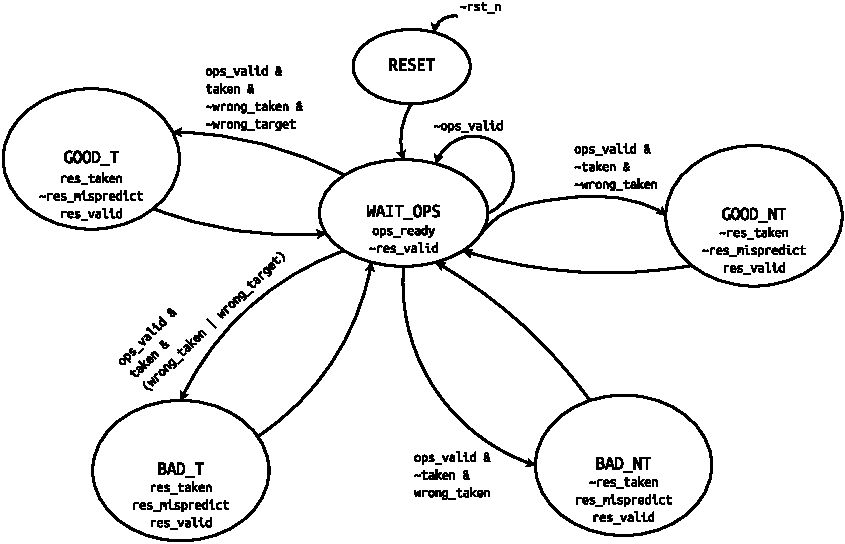
\includegraphics[width=\textwidth]{img/branch_unit_fsm.pdf}
  \caption{Branch unit control unit}
  \label{fig:branch_unit_fsm}
\end{figure}
The control unit of this module is a Moore machine that after reset starts waiting for valid operands from the reservation station in the \texttt{WAIT\_OPS} state. When they arrive, in the same clock cycle the datapath performs the required computation, so that according to the value of the control signals, the \acs{FSM} can move to one of the states named \texttt{{GOOD,BAD}\_{T,NT}}, based on whether there was misprediction and whether the branch was actually taken or not. In these states, the correct output signals are driven and then the state machine moves back to the waiting loop.
\todo{Aggiungere timing dopo modifica}

\chapter{Experimental results}
This chapter presents the results obtained from the design, starting from functional verification of the correctness of the implementation, to synthesis and benchmarking. The entire design has been described in SystemVerilog using hierarchical modules and behavioral constructs when possible. This both helps readability and leaves to the EDA tools the freedom of performing optimizations.

Each module has been verified locally using Verilator\footnote{\url{https://www.veripool.org/wiki/verilator}} for linting and Mentor ModelSim Intel FPGA Starter Edition for simulation. Synthesis has been carried out with Synopsys Design Compiler, on the the VLSI server provided by Politecnico di Torino.

\section{Simulation}
The choice of tools mentioned above was made because one of the pros of Verilator is that it has been found to be more verbose than ModelSim when performing syntax check and lint, thus reducing the number of possible issues during compilation and simulation. Moreover, it is completely free and open source, which nicely couples with the philosophy of the LEN5 project.

ModelSim was in the end chosen as the main simulation tool, because it is much more familiar to the designer and the limited time did not allow to learn Verilator for simulation, given that it uses a completely different paradigm, based on translating HDL to C language and using testbench templates in C as well.

The following sections focus on the test strategies used for the \ac{BPU}, which is almost as important as a standalone design, and the top-level frontend.

\subsection{\acs{BPU}}
The testbench of the \ac{BPU} is based on reading branch addresses from one file, predicting the outcome and then comparing it with the correct branch resolutions coming from a second file. One clock cycle passes between the prediction and the resolution, as to simulate the execution delay, which always takes more cycles. During this time span, the \ac{PC} is fictionally increased to simulate a normal sequential fetch situation.

Given that the length of the history register in the gshare and the length of \ac{BTB} address lead to an exponential growth of the \ac{PHT} and the \ac{BTB} itself, simulations were performed using a small number of bits for these data structures and in particular the following results refer to a configuration with a 4-bit history register and a 4-bit \ac{BTB} address. The simulation is needed to verify the correctness of the design and not the prediction performances, so having fewer bits poses no issues.

In order to test the \ac{BPU} as a singular unit, without all the surrounding processor and in particular without a register file and execution units, some specific test cases have been defined, where branch results could be derived manually without actually executing the program. Loops, in particular, suit well such simple cases.

\subsubsection{Single loop}
The first test case corresponds to the following simple loop:
\begin{lstlisting}[language=C]
  for (int i = 0; i < 10; i++)
  {
    /* loop body */
  }
\end{lstlisting}
Here, the loop condition is tested ten times as true, so the branch is taken, and the last time as false, so the branch is not taken.

\begin{sidewaysfigure}[p]
  \centering
  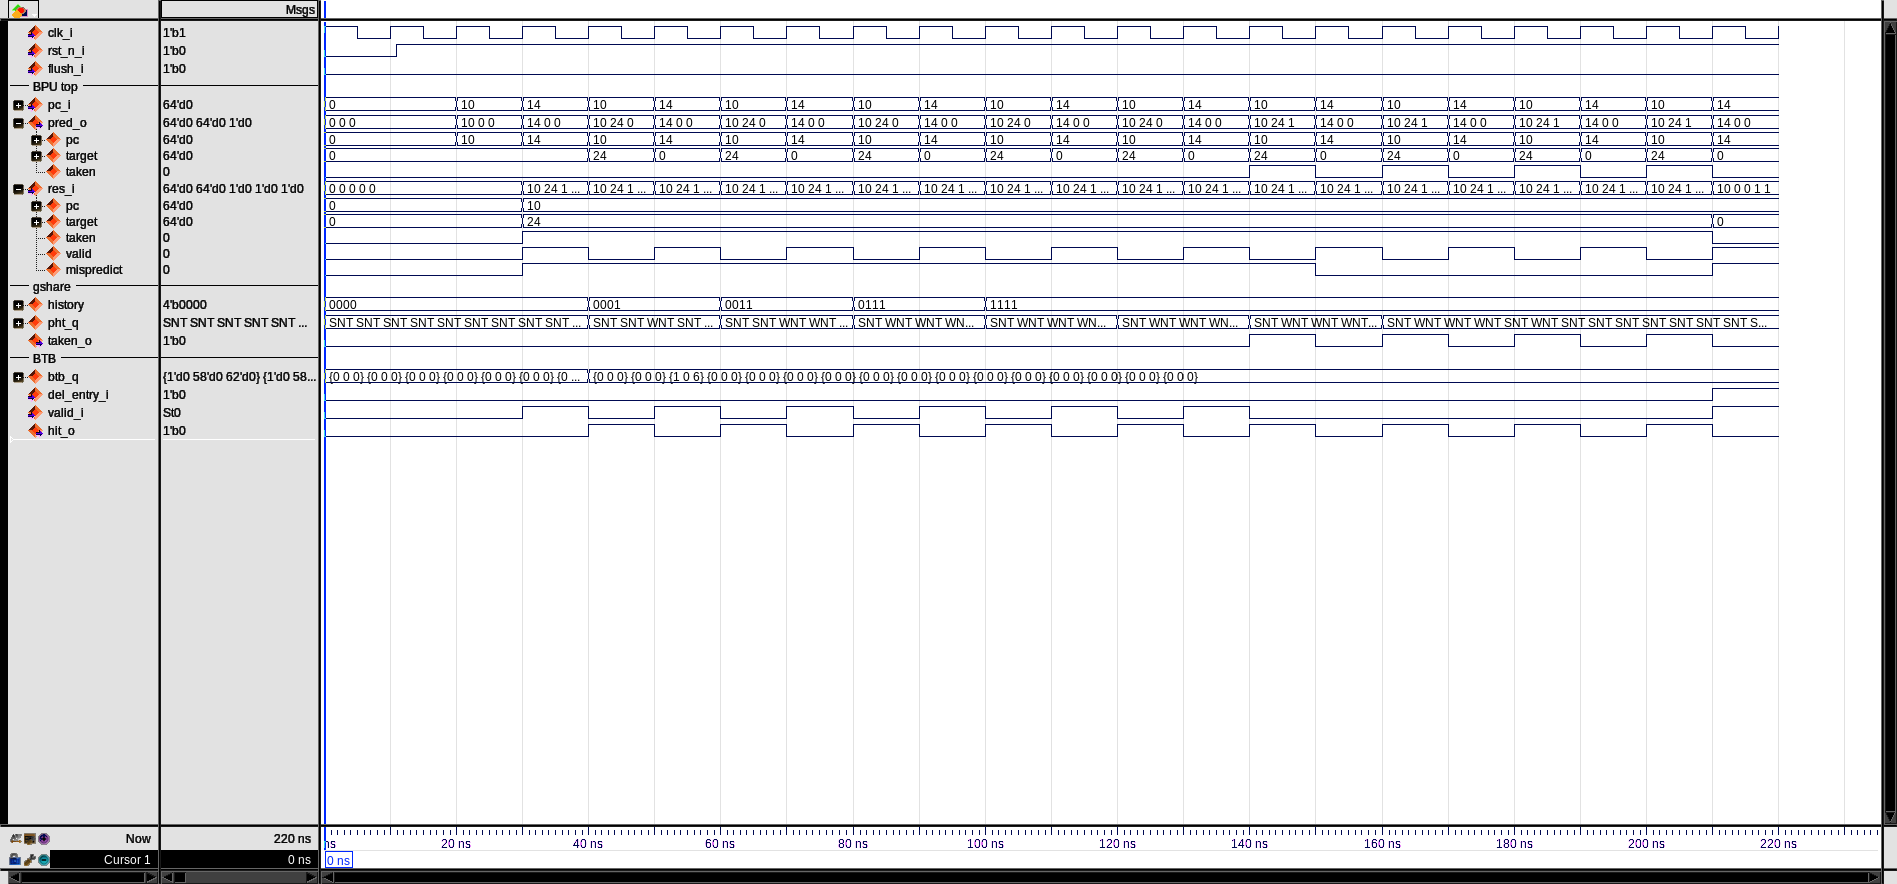
\includegraphics[width=\textheight]{img/bpu_loop01_conv.png}
  \caption{Single loop simulation}
  \label{fig:bpu_loop01_conv}
\end{sidewaysfigure}
Suppose that the instruction testing the loop condition is at address 10 and the beginning of the loop body (i.e.\ the target of the branch instruction) is at address 24. \Cref{fig:bpu_loop01_conv} shows the simulation waveforms for this test case, with the predictions contained in the \texttt{pred\_o} signal, occurring each time the \ac{PC} 10 is read from the address file, and the resolutions read into \texttt{res\_i} every time the \texttt{valid} signal is asserted.

Here, the initialization of the predictor structures can be clearly noted. Given that the history register is initialized to zero and the loop branch is always taken at first, the gshare predictor will initially update 2-bit counters which do not correspond to the actual branch history, until the \ac{BHT} is filled with ones (4 iterations, for the 4-bit register). Then the \ac{PHT} index will remain the same and so the same 2-bit counter is incremented from the initial strongly not taken state to the weakly taken state when it finally starts predicting correctly (2 iterations).

At the seventh iteration of the loop, the branch is predicted correctly as taken (the \texttt{mispredict} signal is deasserted) and this situation lasts until the the loop condition is tested false at the last iteration, leading to a new misprediction. 

Meanwhile, the \ac{BTB} is updated with the correct target at the first iteration, from which it gets a hit each following time.

This \emph{warm-up} of the predictor is intrinsic of its design and cannot be avoided, but anyway \cref{fig:bpu_loop01_conv} demonstrates the correct and expected behavior of the \ac{BPU}.

\subsubsection{Nested loops}
Next, the case of two nested loops was tested, as in the following code:
\begin{lstlisting}[language=C]
  for (int i = 0; i < 20; i++)
  {
    for (int j = 0; j < 3; j++)
    {
      /* loop body */
    }
  }
\end{lstlisting}
This example, actually taken from \cite{mcfarling93}, is intended to demonstrate that the gshare predictor, after the warm-up, can correctly identify taken branches in nested loops, where the outer loop is repeated many times.

\begin{sidewaysfigure}[p]
  \centering
  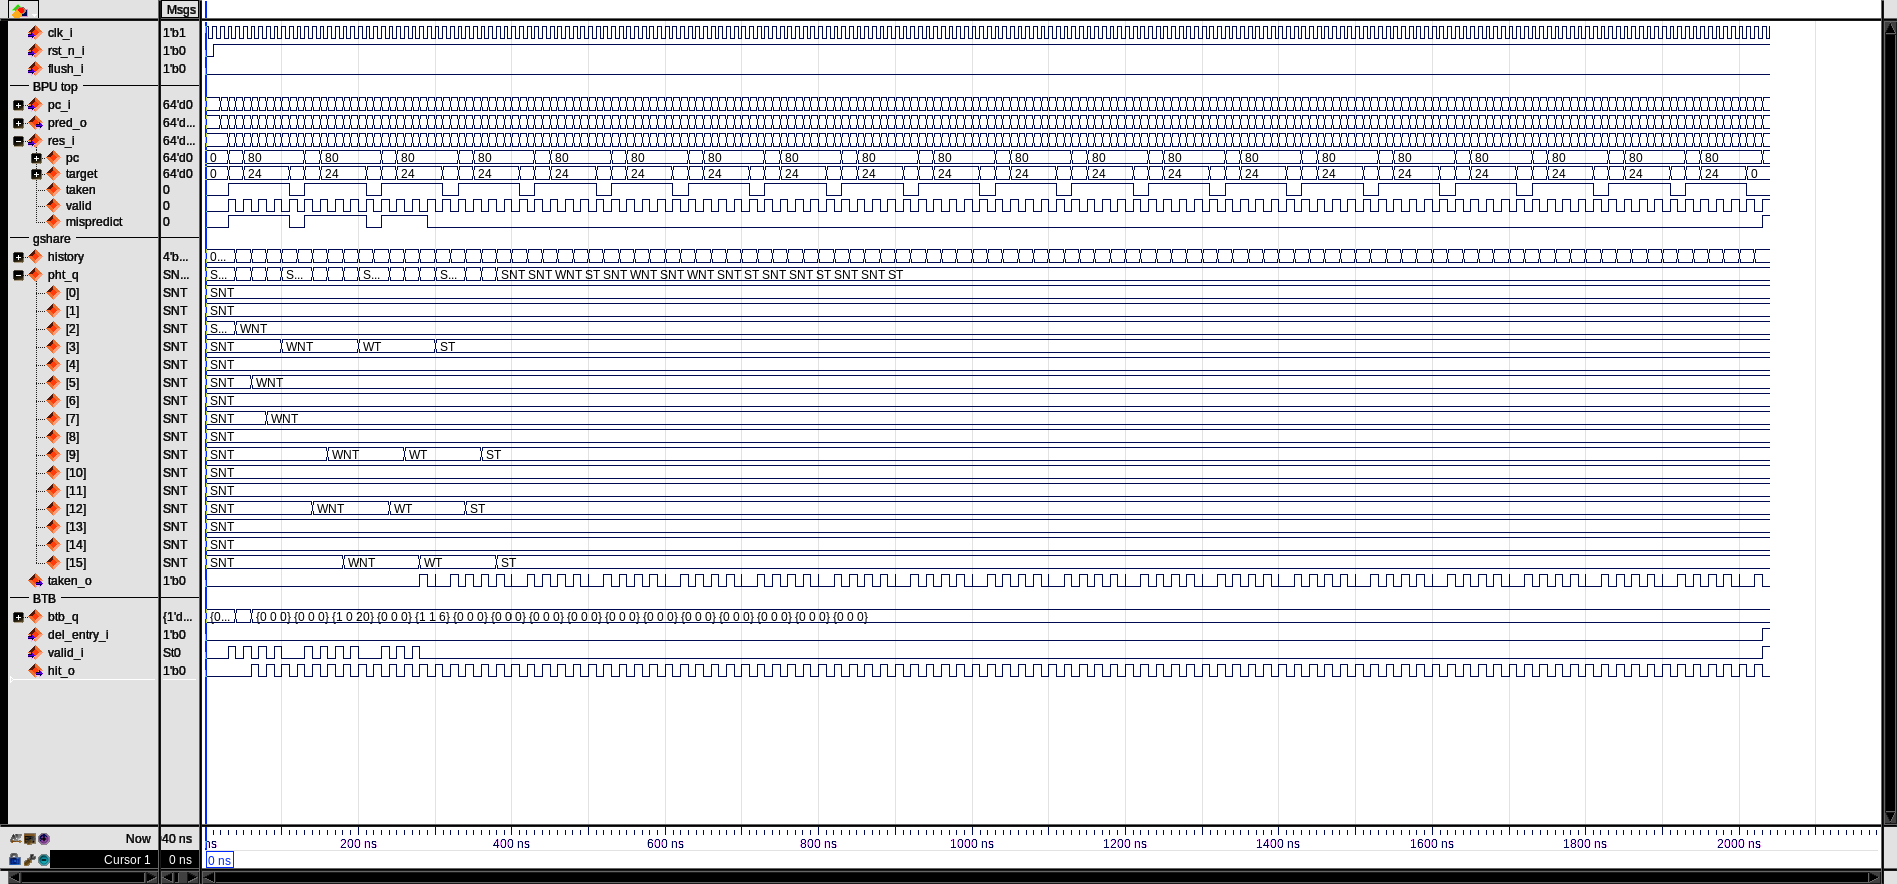
\includegraphics[width=\textheight]{img/bpu_loop02_conv.png}
  \caption{Nested loops simulation}
  \label{fig:bpu_loop02_conv}
\end{sidewaysfigure}
\Cref{fig:bpu_loop02_conv} shows the simulation results for this case, where the address of the condition instruction of the outer loop is 10, the one of the inner loop (i.e.\ the target of the outer loop) is 80 and the body of the inner loop starts at address 24. 

At the beginning, the gshare continuously mispredicts the outer loop and the first iterations of the inner loop, due to the initialization of the \ac{PHT} as mentioned in the previous case, but then after the warm-up it goes on to predict correctly both loops, until the exit of the outer loop. In particular, the steady state situation is shown in \cref{tab:nested}, where each combination of address and history univocally determines the prediction outcome.
\begin{table}[hbt]
  \centering
  \begin{tabular}{lllll}
    \toprule
    \textbf{Value} & \textbf{Condition} & \textbf{\ac{PC}} & \textbf{History} & \textbf{Prediction} \\ \midrule
    \texttt{j = 0} & \texttt{j < 3}   & 80  & 1101  & Taken     \\ \midrule
    \texttt{j = 1} & \texttt{j < 3}   & 80  & 1011  & Taken     \\ \midrule
    \texttt{j = 2} & \texttt{j < 3}   & 80  & 0111  & Taken     \\ \midrule
    \texttt{j = 3} & \texttt{j < 3}   & 80  & 1111  & Not taken \\ \midrule
    \texttt{i = n} & \texttt{i < 20}  & 10  & 1110  & Taken     \\
    \bottomrule
  \end{tabular}
  \caption{Nested loops steady state predictions}
  \label{tab:nested}
\end{table}

\subsection{Frontend}
The testbench designed for the whole frontend is composed of the following blocks that drive its inputs:
\begin{itemize}
  \item A \emph{\ac{PC} jumper} used to simulate exceptions and branches by modifying the sequential generation of addresses.
  \item A \emph{dummy instruction cache} which responds to memory access requests by simulating both hits and misses, with random delays. The fictional data line it provides always contains the \ac{PC} that generated the request and $N$ instruction fields with the number from 1 to $N$ in order to track the movement of instructions.
  \item A \emph{dummy issue queue} that simply simulates a busy issue queue by introducing random delays on the \texttt{issue\_ready} signal.
\end{itemize}

Using this setup, the frontend was simulated in a number of scenarios corresponding to the different situations analyzed in \cref{sec:frontend_timings}, of which the most significant are described below.

\Cref{fig:fetch01_conv} shows the standard situation where subsequent instructions are selected among the same line, saved in the line register after the first memory access at startup (compare with \cref{fig:fetch01}).

\Cref{fig:fetch02_address_conv,fig:fetch02_miss_conv} show the situation of a cache not ready to receive the address or a cache miss respectively, as in \cref{fig:fetch02}. Note also the current states of the instruction cache interface \acs{FSM} that correspond to the timing diagrams of \cref{fig:cache02,fig:cache03}\footnote{These simulation waveforms show \texttt{WAIT\_ADDR} as the wrong old name for the \texttt{WAIT\_REQ} state.}.

\Cref{fig:fetch07_conv} shows a sequence of cache reads in a pipeline fashion, just as in \cref{fig:fetch07}. Note also how here there is a jump right after the boot address, which is correctly handled by the instruction cache interface.

\Cref{fig:fetch09_conv}, like \cref{fig:fetch09}, show the case when the instruction is selected among the line backup register, due to a jump back and forth to the same cache line.

Finally as an example, \cref{fig:fetch03_conv} shows the situation in which the issue queue is not ready during instruction selection (compare with \cref{fig:fetch03}).

\begin{sidewaysfigure}[p]
  \centering
  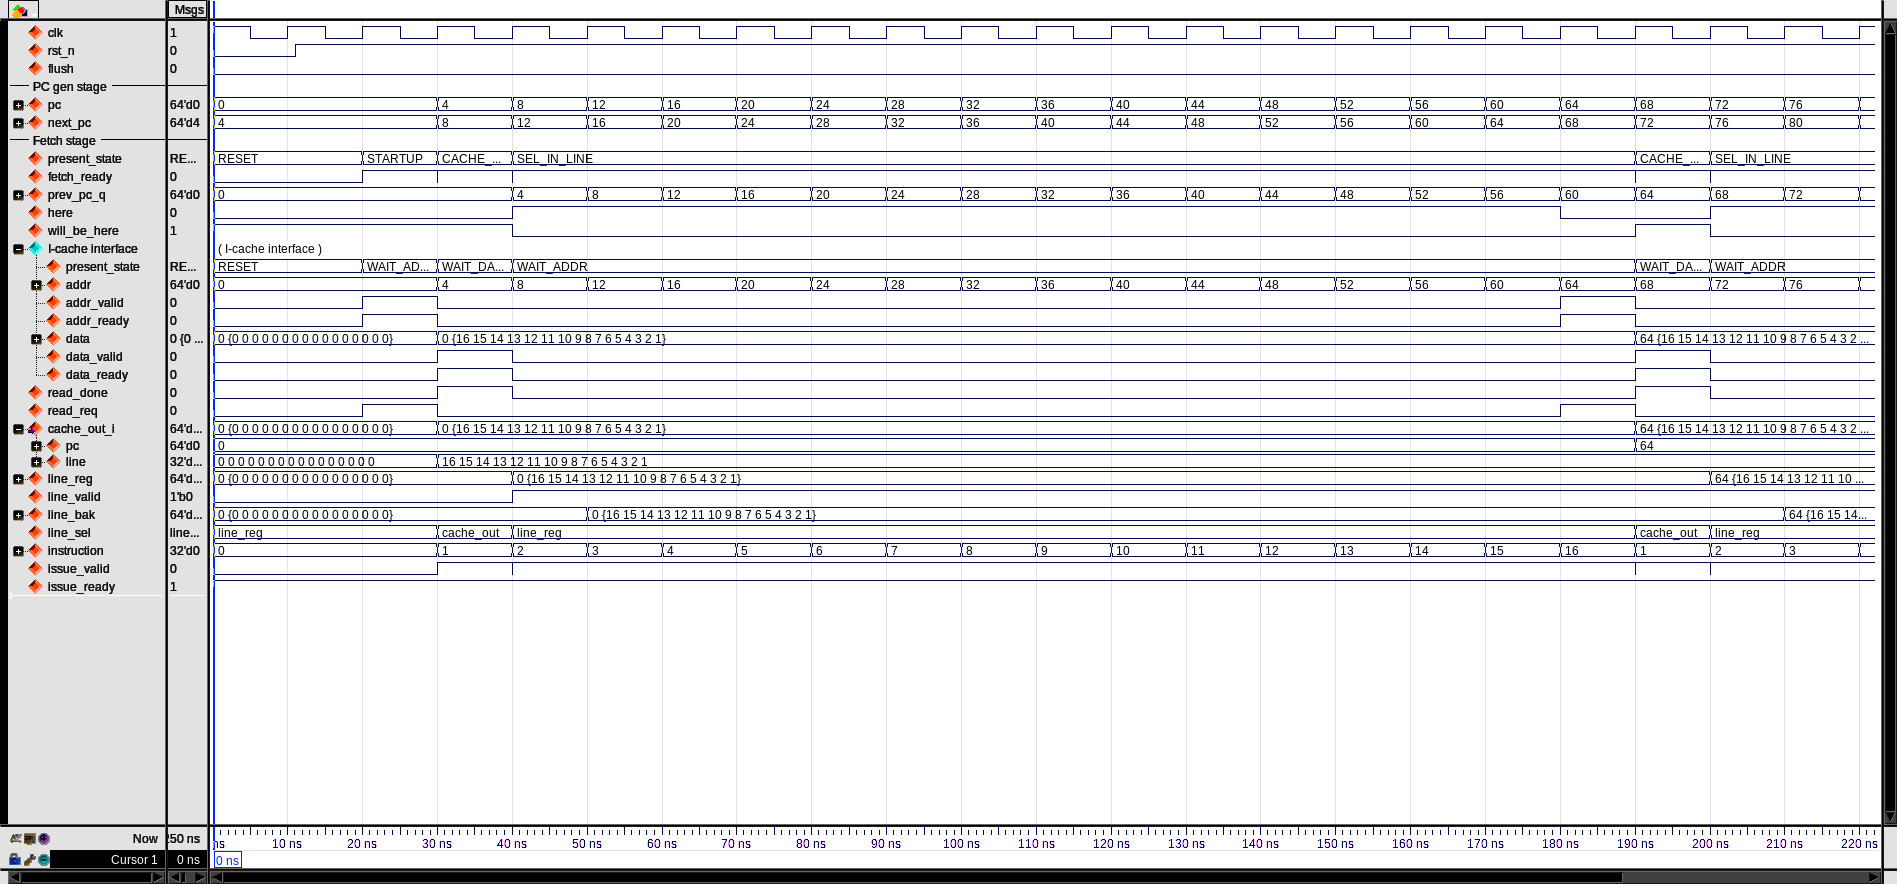
\includegraphics[width=\textheight]{img/fetch01_conv.png}
  \caption{Sequential reads from the same line}
  \label{fig:fetch01_conv}
\end{sidewaysfigure}
\begin{sidewaysfigure}[p]
  \centering
  \includegraphics[width=\textheight]{img/fetch02_address_conv.png}
  \caption{Cache not ready on address}
  \label{fig:fetch02_address_conv}
\end{sidewaysfigure}
\begin{sidewaysfigure}[p]
  \centering
  \includegraphics[width=\textheight]{img/fetch02_miss_conv.png}
  \caption{Cache miss}
  \label{fig:fetch02_miss_conv}
\end{sidewaysfigure}
\begin{sidewaysfigure}[p]
  \centering
  \includegraphics[width=\textheight]{img/fetch07_conv.png}
  \caption{Cache read pipeline}
  \label{fig:fetch07_conv}
\end{sidewaysfigure}
\begin{sidewaysfigure}[p]
  \centering
  \includegraphics[width=\textheight]{img/fetch09_conv.png}
  \caption{Line backup register selection}
  \label{fig:fetch09_conv}
\end{sidewaysfigure}
\begin{sidewaysfigure}[p]
  \centering
  \includegraphics[width=\textheight]{img/fetch03_conv.png}
  \caption{Issue queue busy}
  \label{fig:fetch03_conv}
\end{sidewaysfigure}

\section{\acs{BPU} benchmarking}
As mentioned before, the \ac{BPU} is one of the most configurable units in the design, where a number of parameters and design choices come into play. For this reason a software model of this module written in C has been developed, to allow for fast and simple exploration and benchmarking. The model implements the same functions as the hardware and reads an input text file in the form
\begin{center}
  \texttt{<BRANCH ADDRESS>}  \texttt{<OUTCOME>}
\end{center}
where the address is expressed in hexadecimal base and the outcome as 1 or 0 if the branch is taken or not.

After significant efforts spent to find a way to extract \emph{branch traces} (i.e.\ the list of branch instructions and their result) from a compiled program, no feasible solution was found and so a decision was made to rely on the trace files provided by a laboratory exercise of the course \emph{Principles in Computer Architecture} held by Prof. Dean Tullsen of the University of California San Diego, available on GitHub\footnote{\url{https://github.com/prodromou87/CSE240A}}. These traces come from a series of benchmarks taken from the SPEC suite, listed in \ref{tab:benchmarks}.
\begin{table}[hbt]
  \centering
  \begin{tabular}{lll}
    \toprule
    \textbf{Name}   & \textbf{Type}    & \textbf{Branches}  \\ \midrule
    \texttt{fp\_1}  & Floating point   & \num{1546797}      \\ \midrule
    \texttt{fp\_2}  & Floating point   & \num{2422049}      \\ \midrule
    \texttt{int\_1} & Integer          & \num{3771697}      \\ \midrule
    \texttt{int\_2} & Integer          & \num{3755315}      \\ \midrule
    \texttt{mm\_1}  & Matrix multiply  & \num{3014850}      \\ \midrule
    \texttt{mm\_2}  & Matrix multiply  & \num{2563897}      \\
    \bottomrule
  \end{tabular}
  \caption{\acs{BPU} benchmarks}
  \label{tab:benchmarks}
\end{table}

Given that these trace files do not contain the target address associated with each branch instruction, the main limitation of the software model is that it does not account for mispredictions caused by the wrong target being stored in the \ac{BTB}. It takes into account, however, the case when a \ac{BTB} too small causes entries to be overwritten frequently, increasing the number of misses and thus mispredictions.

In the following sections, a series of tests is described to evaluate performance and other design metrics on the \ac{BPU}.

\subsection{Gshare}\label{sec:gshare_bench}
For what concerns the gshare predictor, three main parameters can be analyzed:
\begin{itemize}
  \item The length of the history register, which determines the number of 2-bit counters in the \ac{PHT}.
  \item The initial value of those counters, which determines the first predictions for each index.
  \item The presence or not of the valid bit, along with each counter.
\end{itemize}

\subsubsection{2-bit counters initialization}
In order to find the best initial value for the counters, each benchmark was run on two different history register lengths (8 and 16 bits) at each possible initialization, including the alternate version even index/weakly not taken odd index/weakly taken.
\begin{table}[hbt]
  \centering
  \begin{tabular}{lllllll}
    \toprule
    \multirow{2}{*}{\textbf{Initial value}} & \multicolumn{6}{c}{\textbf{Benchmark}}                             \\
    \cmidrule{2-7}
                                   & \texttt{fp\_1}               & \texttt{fp\_2}                & \texttt{int\_1}               & \texttt{int\_2}               & \texttt{mm\_1}                & \texttt{mm\_2}                \\
    \midrule
    SNT                            & 98.35\%                      & 88.62\%                       & 69.09\%                       & \cellcolor{cell_blue}98.75\%  & \cellcolor{cell_blue}77.50\%  & 82.37\%                       \\
    WNT                            & 98.36\%                      & 88.55\%                       & 69.09\%                       & 98.75\%                       & 77.50\%                       & \cellcolor{cell_blue}82.37\%  \\
    WT                             & 98.36\%                      & \cellcolor{cell_blue}89.90\%  & \cellcolor{cell_blue}69.09\%  & 98.74\%                       & 77.49\%                       & 82.37\%                       \\
    ST                             & 98.27\%                      & 89.90\%                       & 69.09\%                       & 98.74\%                       & 77.50\%                       & 82.37\%                       \\
    even/WNT, odd/WT               & \cellcolor{cell_blue}98.36\% & 88.65\%                       & 69.09\%                       & 98.74\%                       & 77.50\%                       & 82.37\%                       \\
    \bottomrule
  \end{tabular}
  \caption{Gshare accuracy on different initializations (8-bit history register)}
  \label{tab:init8}
\end{table}
\begin{table}[hbt]
  \centering
  \begin{tabular}{lllllll}
    \toprule
    \multirow{2}{*}{\textbf{Initial value}} & \multicolumn{6}{c}{\textbf{Benchmark}}                             \\
    \cmidrule{2-7}
                                   & \texttt{fp\_1}               & \texttt{fp\_2}                & \texttt{int\_1}               & \texttt{int\_2}               & \texttt{mm\_1}                & \texttt{mm\_2}                \\
    \midrule
    SNT                            & 99.15\%                      & 99.03\%                       & \cellcolor{cell_blue}89.24\% & 99.63\%                        & \cellcolor{cell_blue}96.05\%  & 92.28\%                       \\
    WNT                            & \cellcolor{cell_blue}99.17\% & 98.85\%                       & 88.26\%                      & \cellcolor{cell_blue}99.64\%   & 95.86\%                       & 92.83\%                       \\
    WT                             & 99.16\%                      & \cellcolor{cell_blue}99.04\%  & 89.11\%                      & 99.64\%                        & 95.88\%                       & \cellcolor{cell_blue}92.87\%  \\
    ST                             & 99.15\%                      & 99.04\%                       & 89.23\%                      & 99.61\%                        & 95.97\%                       & 92.39\%                       \\
    even/WNT, odd/WT               & 99.17\%                      & 99.04\%                       & 88.65\%                      & 99.64\%                        & 95.88\%                       & 92.84\%                       \\ 
    \bottomrule
  \end{tabular}
  \caption{Gshare accuracy on different initializations (16-bit history register)}
  \label{tab:init16}
\end{table}

The results are summarized in \cref{tab:init8,tab:init16} for 8-bit and 16-bit history registers respectively, where blue cells represent the best accuracy achieved for each benchmark. It is clear that there is no single best initialization value for the 2-bit counters, but it depends heavily on both the benchmark and the history length. Even the most complex initialization to be performed in hardware, which is the alternate one, results the best only in a single case. In any case, there is not much of a difference among the various initial values, so the conclusion is to choose the simplest one, namely the strongly not taken state (i.e.\ 2-bit counters at zero).

\subsubsection{Valid bit}
From the results of the previous analysis, it is obvious that the valid bit serves no purpose whatsoever in this design. A valid bit would be used to indicate that the indexed counter has been used before and so the prediction is valid. By initializing the 2-bit counters to zero, however, the first (and second) time they are read, they are always going to predict not taken, exactly like the case with the valid bit. In the end, this bit would only increase by 50\% the total \ac{PHT} size, thus literally wasting a significant amount of area.

\subsubsection{History register length}
In order to find the best trade-off between the predictor accuracy and the size of the \ac{PHT}, all the benchmarks were run at increasingly longer history length.
\begin{figure}[hbt]
  \centering
  \includegraphics[width=\textwidth]{img/pht_size.pdf}
  \caption{History register length versus predictor accuracy}
  \label{fig:pht_size}
\end{figure}

From the plot of \cref{fig:pht_size}, the majority of the benchmarks saturate at their best accuracy value in the range between 13 and 20 bits, with only \texttt{int\_1} and \texttt{mm\_1} being the exceptions that continue to get better results the longer the history. 

Given the exponential relation between the history register length and the area of the \ac{PHT}, this range of lengths corresponds to table sizes going from \SI{2}{KB} to \SI{200}{KB}. For this reason, the final value must be chosen by keeping in mind a clear area budget for the final implementation. Having said that, a history length of 16 bits, corresponding to around \SI{16}{KB} of \ac{PHT}, seems like a reasonable compromise for which benchmark results are no more than 2\% worse than the best.

\subsection{\acs{BTB}}
The \ac{BTB} on its own does not contribute to improving the overall prediction accuracy, which only comes from the gshare predictor itself, but instead removes the target computation latency from branch instructions. Thus, its presence can only lower the prediction accuracy with respect to the baseline of the gshare alone, because additional mispredictions are inserted due to \ac{BTB} misses, which occur when the \ac{BTB} does not have a valid entry for the selected address. Moreover, mispredictions take place even when the stored target is then discovered as incorrect, but as mentioned above the available branch traces do not contain the correct target, so the software model does not take this kind of mispredictions into account, which contribute only in small part anyway.
\begin{figure}[hbt]
  \centering
  \includegraphics[width=\textwidth]{img/btb_size.pdf}
  \caption{\acs{BTB} index size versus MPKI}
  \label{fig:btb_size}
\end{figure}

\Cref{fig:btb_size} shows the results of the benchmarks with varying length of the \ac{BTB} index expressed as the number of mispredictions per a thousand instructions (MPKI), where dashed lines represent the baseline without \ac{BTB} for each benchmark. Some programs, like \texttt{mm\_1} and \texttt{mm\_2} suffer significantly with small \acs{BTB} and have unacceptably high misprediction rates, while other, notably \texttt{int\_2} seem almost unaffected by the presence of the \ac{BTB}. Anyway, around 10 or 12 bits for the \ac{BTB} index, i.e.\ in the range \SI{15}{KB} to \SI{60}{KB}, most of the benchmark have reached a MPKI very close to the baseline. Going past these values does not seem to offer a significant improvement and thus becomes unadvisable, regardless of the area constraints.

\section{Synthesis}
Synthesis has been carried out using Synopsys Design Compiler on the UMC \SI{65}{nm} low leakage (L65LL) technology library. In order to get reproducible results, scripting was heavily used to input commands to the tool and some notable parameters and settings used in the process are listed below:
\begin{itemize}
  \item Top down compilation, to allow optimizations beyond module boundaries, even if this means potentially longer compile times and higher memory usage, as stated in \cite[p.8-6]{dc}.
  \item Ideal clock definition (\texttt{set\_ideal\_network} and \texttt{set\_dont\_touch\_network}) in order to avoid optimizations on the clock tree, which has to be defined in later place and route stages, and remove warnings about its high fanout.
  \item Clock uncertainty (skew) \SI{0.07}{ns}
  \item Maximum input and output delay \SI{0.5}{ns}
  \item Output load of a buffer on all ports (\texttt{BUFM10R}, \SI{2.1}{\femto\farad})
  \item DC Expert compilation (\texttt{compile} command)
\end{itemize}

\subsection{\acs{BPU}}
The \ac{BPU} was synthesized in different configurations of history register length and \ac{BTB} size, in order to evaluate the effect of these parameters variations on the design metrics. In particular, from the considerations and the results obtained during benchmarking, the history length was varied between 2 and 16 bits and the \ac{BTB} index length from 2 to 12 bits. Given that the size of the \ac{BPU} grows exponentially with both these parameters, the syntheses, executed with a batch script, took several days to complete.

\subsubsection{Area}
The total area of the \ac{BPU} depends almost exclusively on the size of the gshare \ac{PHT} and the \ac{BTB}, which are determined by the history length and the \ac{BTB} index bits. More specifically, given that each entry of the \ac{BTB} easily contains more than 100 bits compared to the 2 bits of a \ac{PHT} entry, the effect of the \ac{BTB} size will weigh 100 times more than the history length on the overall result. In other words, the length of the history register matters only with small \acp{BTB}, while it becomes negligible alongside large buffers.

\begin{figure}[hbt]
  \centering
  \includegraphics[width=\textwidth]{img/bpu_area.pdf}
  \caption{Total \acs{BPU} area versus history length and \ac{BTB} size}
  \label{fig:bpu_area}
\end{figure}
This effect is evident in \cref{fig:bpu_area}, which shows the synthesized values of total cell area, demonstrating the expected exponential growth (linear on this logarithmic $z$ axis) with respect to the length of the \ac{BTB} index. The history length has the effect of slightly increasing the cell area (bending the plane) for low values of the \ac{BTB} bits, but that effect vanishes for larger buffers and in the end the final area in the case of large \acp{BTB} is constant regardless of history length.

Actually, for such large predictor structures, an implementation as register files becomes infeasible and the better way to synthesize them would be to use a memory compiler and a small SRAM to store the \ac{PHT} and \ac{BTB}.

\subsubsection{Timing}
For what concerns timing, the critical path was reported to be the \ac{BTB} and in particular the path going from the \ac{BTB} address part of the \ac{PC} to the \texttt{hit} signal, to the \texttt{taken} output. Presumably, this corresponds to the decoding network inferred to correctly select the \ac{BTB} entry. For this reason, \ac{BTB} size and thus the complexity of such decoder was consistently reported as the only timing critical part of the design, while no variation whatsoever was noted increasing the history bits.

\begin{figure}[hbt]
  \centering
  \includegraphics[width=\textwidth]{img/bpu_freq.pdf}
  \caption{Maximum \acs{BPU} clock frequency versus \ac{BTB} index bits}
  \label{fig:bpu_freq}
\end{figure}
\Cref{fig:bpu_freq} shows the results of the maximum achievable clock frequency, obtained by setting the target clock period to zero, with increasing \ac{BTB} index bits used. Between the two extremes, the critical path grows of about \SI{0.6}{ns}, which correspond to a non-negligible drop of about \SI{200}{MHz} in maximum frequency. The seemingly linear negative trend can be explained by reckoning that the decode network to address the \ac{BTB} is likely to be implemented as a balanced tree of logic gates, whose number of levels thus depends on the base-2 logarithm of the number of entries of the buffer, which in turn grows exponentially with the number of bits, leading to a linear dependence.

In the end, the actual size of the \ac{BTB} must be chosen by keeping into account the design constraints both in terms of area budget and of target clock frequency, trading them off with the prediction accuracy and hit rate. History bits, on the other hand, do not influence timing at all.

\subsection{Frontend}
\chapter{Concluding remarks}

\section{Future work}

%%% Bibliography %%%
\begin{thebibliography}{99}
\setlength{\parskip}{0.5\baselineskip}

\bibitem{waterman}
    Waterman A., 
    \textit{Design of the RISC-V Instruction Set Architecture},
    PhD diss.,
    Electrical Engineering and Computer Sciences,
    University of California at Berkeley,
    2016,
    UCB/EECS-2016-1.

\bibitem{reader}
    Patterson D., Waterman A., 
    \textit{The RISC-V Reader: An Open Architecture Atlas},
    First edition,
    Strawberry Canyon,
    2017.

\bibitem{hennessy17}
    Hennessy J., Patterson D., 
    \textit{Computer Architecture: A Quantitative Approach},
    Sixth edition,
    Morgan Kaufmann,
    2017.

\bibitem{scoreboard}
    Thornton J.,
    ``Parallel operation in the control data 6600'',  
    \textit{Proceedings of the October 27–29, 1964, fall joint computer conference, part II: very high speed computer systems},
    vol. 26, pp. 33-40, 
    1965.

\bibitem{mittal19}
    Mittal S.,
    ``A Survey of Techniques for Dynamic Branch Prediction'',  
    \textit{Concurrency and Computation: Practice and Experience},
    vol. 31, no. 1, 
    2019.
    
\end{thebibliography}

\end{document}